\documentclass[11pt, a4paper]{article}


\usepackage[top=1 in, bottom = 1 in, left = 1 in, right = 1 in ]{geometry}

\usepackage{amsmath, amssymb, amsfonts}
\usepackage{hyperref}

\usepackage{polyglossia}

\usepackage{fontspec}

\usepackage{enumerate}

\usepackage{graphicx}

\usepackage{float}


\setdefaultlanguage{english}
\setotherlanguage{bengali}


\newfontfamily{\bengalifont}[Script=Bengali]{kalpurush.ttf}


\begin{document}

\tableofcontents
\pagebreak


	
\section{Logarithm}

\begin{enumerate}


%01
     \item Solve for x : $ \log_x 3 \cdot \log_{\frac{x}{81}} 3 = \log_{\frac{x}{729}} 3. $

%02
	\item \textbengali{যদি} 
		$ y= 10 ^ {\dfrac{1}{1-\log_{10} x}}, z= 10 ^ {\dfrac{1}{1-\log_{10} y}} $ 
		\textbengali{হয়, তবে প্রমাণ কর যে,}
		$ x= 10 ^ {\dfrac{1}{1-\log_{10} z}}.$
 
%03   
     \item \textbengali {যদি} $ x = \dfrac{e^y - e^{-y}}{e^y + e^{-y}} $ \textbengali {হয়, তবে দেখাও যে,} $ y = \dfrac{1}{2} \log_e \dfrac{1+x}{1-x}. $
     

%04
     \item \textbengali{মান নির্ণয় কর }:- $ \log_6 \sqrt{6\sqrt{6\sqrt{6 \cdots \cdots \infty}}}. $
     
%05
     \item \textbengali{প্রমাণ কর যে,} $ \log_{10} 2 > 0.3 $.
     
%06
     \item \textbengali {যদি} $ \dfrac{\log x}{ry - qz} = \dfrac{\log y}{pz - rx} = \dfrac{\log z}{qx - py} $ \textbengali{হয়, তবে প্রমাণ কর যে} $ x^p y^q z^r = 1 $.
     
%07
     \item $ \log_p x = a $, $ \log_q x = b $ \textbengali{হলে দেখাও যে,} $ \log_{\frac{p}{q}} x = \dfrac{ab}{b-a} $.
     
%08
     \item \textbengali{যদি} $ \log_a b = 10 $ \textbengali{ও} $ \log_{6a} 32b = 5 $ \textbengali{হয় তবে} $a$ \textbengali{ও} $b$ \textbengali{এর মান কত?}
     
%09
     \item $ x = \log_a bc$, $ y = \log_b ca $, $ z = \log_c ab $ \textbengali{হলে দেখাও যে}
     		\begin{enumerate}[(i)]
     		\item $ \dfrac{1}{x+1} + \dfrac{1}{y+1} + \dfrac{1}{z+1} = 1 $.
     		\item $ x+y+z = xyz - 2 $.
     		\end{enumerate}
     		
%10
     	\item If $ \log (x^2y^3) = a $ and $ \log \left(\dfrac{x}{y}\right) = b $, find $\log x $ and $\log y $ in terms of $a$ and $b$. 
     	
%11
     	\item Solve :- $\log_4 (x-1) = \log_2 (x-3) $.
     	
%12
     	\item Solve :- $ \log_{(2x+3)} \left( 6x^2 + 23x + 21 \right) + \log_{(3x+7)} \left( 4x^2 + 12x + 9 \right) = 4 $.
     	
%13
     	\item If $ \log_{10} 2 = 0.30103 $, $\log_{10} 3 = 0.47712$, and $\log_{10} 7 = 0.84510 $, find the values of \begin{enumerate}[(i)]
     		\item $ \log_{10} 45 $
     		\item $ \log_{10} 105 $
     	\end{enumerate}
     	
%14
     	\item Prove that, $ \log_2 10 - \log_8 125 = 1 $.
     	
%15
     	\item Show that, $ a^{\log_{a^2} x} \cdot b^{\log_{b^2} y} \cdot c^{\log_{c^2} z}  = \sqrt{xyz}$.
     	
%16
     	\item If $ \log_2 x + \log_4 x + \log_{16} x = \dfrac{21}{4} $, find the value of x.
     	
%17
     	\item Prove that, $ (yz)^{\log \dfrac{y}{z}} \cdot (zx)^{\log \dfrac{z}{x}} \cdot (xy)^{\log \dfrac{x}{y}} = 1 $.
     	
%18
     	\item Show that, $ \dfrac{1}{\log_a bc + 1} + \dfrac{1}{\log_b ca + 1} + \dfrac{1}{\log_c ab + 1} = 1 $.
     	
%19
     	\item Solve : $ \log_5 (5^{\frac{1}{x}} + 125) = \log_5 6 + 1 + \dfrac{1}{2x} $.
     	
%20
     	\item If $a>0$; $c>0$; $b=\sqrt{ac}$; $a$, $c$ and $ ac \neq1  $; $N>0$; prove that, \begin{center}
     	
     	
     $\dfrac{\log_a N}{\log_c N} = \dfrac{\log_a N - \log_b N}{\log_b N - \log_c N}$.
     \end{center}
     
%21
     \item If $ \dfrac{r}{r_1} + \log_e \dfrac{r_2}{r_1} = 1 $ and $ r_2 = er $, then show that, $ \dfrac{r_1}{r} \log_e \dfrac{r_1}{r} = 1 $.
     
%22
     \item If $ \dfrac{\log a}{y+z} = \dfrac{\log b}{z+x} = \dfrac{\log c}{x+y} $, then show that, $ \left( \dfrac{b}{c} \right)^x \cdot \left( \dfrac{c}{a} \right)^y \cdot \left( \dfrac{a}{b} \right)^z = 1 $.
     
%23
     \item Solve : $ x^{\log_{10} x} = 100x $.
     
%24
     \item Solve : $ 2\log_2 \log_2 x + \log_{\frac{1}{2}} \log_2 (2\sqrt{2}x) = 1 $.
     
%25
     \item Solve : $ 4^{\log_9 3} + 9^{\log_2 4} = 10^{\log_x 83} $.
     
%26
     \item If $ (\log_b a \cdot \log_c a - \log_a a) + (\log_c b \cdot \log_a b - \log_b b) + (\log_a c \cdot \log_b c - \log_c c) = 0 $, then show that, \begin{enumerate}[(i)]
     		\item $ a=b=c $.
     		\item $ abc = 1 $.
     \end{enumerate}
     
%27
     \item If $ x = 1 + \log_a (bc) $ , $ y = 1 + \log_b (ca) $, $ z = 1 + \log_c (ab) $, prove that, $ xy + yz + zx = xyz $.
     
%28
     \item Show that, $ \dfrac{\log_a x}{\log_{ab} x} = 1 + \log_a b $.
     
%29
     \item If the logarithm of $a^2$ to the base $b^3$ and the logarithm of $b^8$ to the base $a^{12}$ be equal, find the value of each logarithm.
     
%30
     \item Solve : $ \dfrac{1}{\log_x 10} + 2 = \dfrac{2}{\log_{0.5} 10} $ .   
     
%31
     \item Find the value of $ \log_3 2^{\log_4 3^{\log_5 4^{\log_6 5 \cdots \log_{1024} 1023}}} $ 	.
     
%32
     \item Find the value of $ \log_2 1^{\log_3 2^{\log_4 3 \cdots \infty}} $.
     	
%33
     	\item Solve :- $ x^{\log_2 x} + a^{\log_2 x} = 2a^2(a>1) $.
     	
%34
     	\item Prove that, $ a^{\log b} = b^{\log a} $.
     	
%35
     	\item If $ \dfrac{pq\log (pq)}{p+q} = \dfrac{qr\log (qr)}{q+r} = \dfrac{rp\log (rp)}{r+p} $, then prove that, $ p^p = q^q = r^r $.
     	
%36
     	\item If $ \log_{12} 27 = a $ then find the value of $ \log_{6} 16 $ in the terms of $a$.
     	
%37
     	\item If $ x = 10! $, find the value of $ \dfrac{1}{\log_2 x} + \dfrac{1}{\log_3 x} + \dfrac{1}{\log_4 x} + \cdots + \dfrac{1}{\log_{10} x} $.
     	
%38
     	\item Find the value of $ (25)^{\frac{1}{2} + \log_{\frac{1}{5}} 27+ \log_{25} 81} $.
     	
%39
     	\item $ 2\log_{10} x - \log_x (0.01) $ [$x>1$] \textbengali{রাশিটির ক্ষুদ্রতম মান কত}?
     	
%40
     	\item If $ 2 \log_8 N = P $, $ \log_2 2N = q $ and $ q - p = 4 $, find the value of $ N $.
     	
%41
     	\item If $ a = \log_3 5 $  \& $ b = \log_{17} 25 $, show that $ a>b $.
     	
%42
     	\item If $ x^2 + y^2 = z^2 $, prove that, $ \dfrac{1}{\log_{z-y} x} + \dfrac{1}{\log_{z+y} x} = (2+\sqrt{2}) (2-\sqrt{2}) $.
     	
%43
     	\item $ 5^{(2 - \log_5 2)} $ \textbengali{এর মান কত?}
     	
%44
     	\item Prove that, $ \log_a x \cdot \log_b y \cdot \log_c z = \log_b x \cdot \log_c y \cdot \log_a z$.
     	
%45
     	\item Prove that, $ \log (1^{\frac{1}{5}} + 32^{\frac{1}{5}} + 243^{\frac{1}{5}}) = \dfrac{1}{5} \left( \log 1 + \log 32 + \log 243\right) $.
     	
%46
     	\item Prove that, $ \log_a x + \log_{a^2} x^2 + \log_{a^3} x^3 + \log_{a^4} x^4  + \cdots + \log_{a^n}x^n = \log_a x^n$.
     	
%47
     	\item $ \log_3 \sqrt{6} + \log_3 \sqrt{\dfrac{2}{3}} - \log_3 \log_3 9 $ \textbengali{এর মান কত?}
     	
%48
     	\item If $ x + y = z $, prove that, $ \dfrac{1}{\log_{\sqrt{z} - \sqrt{y}} x} + \dfrac{1}{\log_{\sqrt{z} + \sqrt{y}} x} = 1 $.
     	
%49
     	\item Find the value of $ \log_2 \sqrt[4]{64\sqrt[3]{4^{(-1)} 8^{-\frac{4}{3}}}} $.
     	
%50
     	\item If $ x = \log_b a + \log_a b $, $ y = \log_c b + \log_b c $, $ z = \log_a c + \log_c a $; prove that, $ x^2 + y^2 + z^2 - 4 = xyz $.
     	
%51
     	\item If $ \dfrac{a(b+c-a)}{\log a} = \dfrac{b(c+a-b)}{\log b} = \dfrac{c(a+b-c)}{\log c} $, prove that, $ a^b \cdot b^a = b^c \cdot c^b = a^c \cdot c^a $.
     	
%52
     	\item If $ \log_{12} m = a $, $ \log_{18} m = b $, prove that, $ \log_3 2 = \dfrac{a-2b}{b-2a} $.
     	
%53
     	\item Solve:- $ \dfrac{\log_2 (x+4) + 1}{\log_{\sqrt{2}} (\sqrt{x+3} - \sqrt{x-3})} = 1 $.
  
%54
	\item Prove that, the value of $\log_{10} 3$ lies between $ \dfrac{1}{2} $ and $ \dfrac{2}{5} $.
	
%55
	\item Prove that, $ \dfrac{1}{\log_2 \pi} + \dfrac{1}{\log_6 \pi} > 2 $.
	
%56
	\item Solve:- $ \log_7 \log_5 ( \sqrt{x+5} + \sqrt{x} ) = 0 $.
	
%57
	\item Solve:- $ x + \log_{10} ( 1 + 2x ) = x\log_{10} 5 + \log_{10} 6 $.
	
%58
	\item If $ \log_{40} 4 = a $, $ \log_{40} 5 = b $, show that $ \log_{40} 16 = 4(1-a-b) $.
	\begin{center}
	\textbf{OR} 
	\end{center}
	If $ \log_{40} 4 = a $, $ \log_{40} 5 = b $, find the value of $ \log_{40} 16 $ in terms of $a$ \& $b$.
	
%59
	\item If \,  $ \log (a+b+c) = \log a + \log b + \log c $,then prove that,\\ \\ $ \log \left( \dfrac{2a}{1-a^2} + \dfrac{2b}{1-b^2} + \dfrac{2c}{1-c^2} \right) = \log \dfrac{2a}{1-a^2} + \log \dfrac{2b}{1-b^2} + \log \dfrac{2c}{1-c^2} $.
	
%60
	\item If \, $ b = \dfrac{c+a}{2} $ and $ y^2 = zx $, then prove that, 
	\begin{center}
	$ a^{(b-c)\log_a x} \cdot b^{(c-a)\log_b y} \cdot c^{(a-b)\log_c z} = 1 $.
	\end{center}
	
%61
	\item If $ 2 \log_m x = \log_l x + \log_n x $, show that $ \log n^2 = \log (ln) \cdot \log_l m $.
	
%62
	\item If $ b-a = c-b  $ and $ \dfrac{y}{x} = \dfrac{z}{y} $, prove that $ (b-c)\log x + (c-a)\log y + (a-b)\log z = 0 $.
	
%63
	\item If $x$, $y$, $z$ are in G.P., prove that $ \log_a x + \log_a z = \dfrac{2}{\log_y a} $ where $x$, $y$, $z$, $a$ $>$ $0$.
	
%64
	\item If $ \log_6 15 = a $, $ \log_{12} 18 = b $, $ \log_{25} 24 = c $, show that $ c = \dfrac{5-b}{2(ab+a-2b+1)} $.
	
%65
	\item If $ \log_{12} 18 = x $, $ \log_{24} 54 = y$ show that, $ xy + 5(x-y) = 1 $.
	
%66
	\item If $ 2 \log_{10} 2 = (2-a) $, show that, $ \log_{10} 5 = \dfrac{a}{2} $.
	  			 
	  			 
%67
	\item If $ (ax)^{\log a} = (bx)^{\log b} $, show that $x = \dfrac{1}{ab} $.
	
%68
	\item If $\log_{10} 2 = x$, $\log_{10} 3 = y$, show that $\log_{10} 45 = 2y - x + 1$.
	
%69
	\item If $\log_{10} 2 = x$, show that $\log_{8} 25 = \dfrac{2}{3} \left( \dfrac{1}{x} - 1 \right)$.
	
%70
	\item If $a^2 + b^2 = c^2$, show that $\log_{(c-b)} a + \log_{(c+b)} a = 2 \cdot \log_{(c+b)} a \cdot \log_{(c-b)} a$.


\end{enumerate}


\section{Geometry}

\begin{enumerate}
%01

	\item ABC 
			\textbengali{ও}  
			BDC 
			\textbengali{দুটি ত্রিভুজ একই ভূমি} 
			BC
		   \textbengali{-র একই পাশে অবস্থিত।} 
		   AB, AC, CD, BD 
		   \textbengali{বাহুগুলির মধ্যবিন্দু যথাক্রমে} 
		   P,Q,R,S.
		  \textbengali{প্রমাণ কর যে,} 
		     \begin{center}
		     
		      PQRS
		     \textbengali{ সামান্তরিকের ক্ষেত্রফল =}
		  $ \dfrac{1}{2} \left(\bigtriangleup BDC \sim \bigtriangleup ABC \right). $
		     \end{center}
		    
%02 
	\item ABCD, CDEF \textbengali{ও} EFGH \textbengali{হল তিনটি বর্গক্ষেত্র ।} AF \textbengali{ও} BH \textbengali{পরস্পরকে} O \textbengali{বিন্দুতে ছেদ করেছে। প্রমাণ কর যে,} $ \angle HOF = 45^{\circ}. $

%03	
	\item ABCD \textbengali{একটি বর্গক্ষেত্র।}  \textbengali{এর মধ্যে } P \textbengali{এমন একটি বিন্দু যেন}  PB = PC \textbengali{হয়।}   $ \angle PAD = 15^{\circ} $. \textbengali{প্রমাণ কর যে,} \\ PB = BC = PC. 

%04	
	\item ABCD \textbengali{আয়তক্ষেত্রের}  C \textbengali{বিন্দুগামী একটি বৃত্ত}  AB \textbengali{ও}  AD \textbengali{কে যথাক্রমে}  M \textbengali{ও} N \textbengali{বিন্দুতে ছেদ করে।}  MN \textbengali{জ্যা এর উপরে} C \textbengali{বিন্দু থেকে}  CP \textbengali{লম্ব।} \textbengali{প্রমাণ করতে হবে,} ABCD \textbengali{আয়তক্ষেত্রের ক্ষেত্রফল} = (CP)$^2$.

%05	
	\item $\bigtriangleup$ ABC \textbengali{একটি সূক্ষ্মকোণী ত্রিভুজ।}  $\angle BAC = 30^{\circ} $. H \textbengali{লম্ববিন্দু} ; M, BC \textbengali{বাহুর মধ্যবিন্দু।}  H, M \textbengali{যোগ করে} T \textbengali{বিন্দু পর্যন্ত এমনভাবে বাড়ানো হল যাতে}  HM = MT \textbengali{হয়। প্রমাণ করতে হবে,}  AT = 2BC. [INMO 1995]

%06	
	\item Fermat's Point

%07	
	\item $\bigtriangleup$ ABC \textbengali{এর} AD, BE \textbengali{ও} CF \textbengali{তিনটি মধ্যমা পরস্পরকে}  G \textbengali{বিন্দুতে ছেদ করেছে।}   \textbengali{প্রমাণ কর যে, }
	\begin{enumerate}[(i)]
	\item $8(BE)^2 + 8(CF)^2 - 4(AD)^2 = 9(BC)^2$
	\item $8(BE)^2 + 8(AD)^2 - 4(CF)^2 = 9(AB)^2$	
	\item $8(CF)^2 + 8(AD)^2 - 4(BE)^2 = 9(AC)^2$
	\end{enumerate}
	

%08	
	\item Apollonius' Theorem
	

%09
	\item ABC \textbengali{একটি সমদ্বিবাহু ত্রিভুজ।} A \textbengali{বিন্দুগামী} BC \textbengali{এর সমান্তরাল সরলরেখার ওপর} D \textbengali{একটি বিন্দু।} BCD \textbengali{অপর একটি ত্রিভুজ। প্রমাণ কর যে,} $ BD + CD > AB + AC $.
	
%10
	\item $ \bigtriangleup $ ABC \textbengali{এর} AD \textbengali{মধ্যমা।} $ \angle ADB = 45^{\circ} $ \textbengali{ও}  $ \angle ACB = 30^{\circ} $. $ \angle BAD = $ \textbengali{কত?} [RMO 2005]
	
%11
	\item ABC \textbengali{একটি সমকোণী ত্রিভুজ যার} $ \angle ABC = 90^{\circ} $. BCRS, ACXY, AQPB \textbengali{হল তিনটি বর্গক্ষেত্র যাদের প্রতিটি বাহু যথাক্রমে} $ a,c,b $. \textbengali{প্রমাণ করতে হবে,} $ (XR)^2 + (QY)^2 = 5(PS)^2 $.
	
%12
	\item $ \bigtriangleup $ ABC \textbengali{এর} S \textbengali{পরিকেন্দ্র}, O \textbengali{লম্ববিন্দু} , R \textbengali{পরিব্যাসার্ধ হলে প্রমাণ কর যে,} \\ $ (AB)^2 + (BC)^2 + (AC)^2 = 12R^2 - [ (OA)^2 + (OB)^2 + (OC)^2 ] $.
	
	\newpage
	
%13
	\item $ \bigtriangleup $ ABC \textbengali{এর} $ \angle A $, $ \angle B $, $ \angle C $ \textbengali{কোণের বিপরীত বাহু যথাক্রমে} $ a,b,c $ \textbengali{হলে ও } C \textbengali{বিন্দুগামী উচ্চতার দৈর্ঘ্য } $ h $ \textbengali{হলে প্রমাণ কর যে,} \begin{center}
	$ h = \dfrac{\sqrt{(a+b+c)(a+b-c)(b+c-a)(c+a-b)}}{2c} $.
	\end{center}
	
%14
	\item $ \bigtriangleup $ ABC \textbengali{এর} $ \angle A $, $ \angle B $, $ \angle C $ \textbengali{কোণের বিপরীত বাহু যথাক্রমে} $ a,b,c $ \textbengali{হলে ও } C \textbengali{বিন্দুগামী মধ্যমার দৈর্ঘ্য } $ x $ \textbengali{হলে প্রমাণ কর যে,}
\begin{center}
$ x = \dfrac{\sqrt{2a^2 + 2b^2 - c^2}}{2} $.
\end{center}

%15
	\item $ \bigtriangleup $ ABC \textbengali{এর} $ \angle B = 2\angle C $ \textbengali{হলে নিচের কোনটি সঠিক}?
	\begin{enumerate}[(i)]
		\item $ AC <2AB $.
		\item $ AC = 2AB $.
		\item $ AC > 2AB $.
	\end{enumerate}
	
%16
	\item \textbengali{ব্রহ্মগুপ্তের সূত্র - ত্রিজুজের পরিব্যাসার্ধ নির্ণয়}
	
%17
	\item $ ABCD $ \textbengali{সামান্তরিক}, $ BQ \perp AD $ \textbengali{হলে প্রমাণ কর যে,}  $ (AC)^2 - (BD)^2 = 4 (AQ) (AD) $.
	
%18
	\item $ \bigtriangleup ABC $ \textbengali{এর} $ \angle BAC $ \textbengali{এর সমিদ্বখণ্ডক} $ AE $, $ AD \perp AE $. Prove that, $ AB + AC < BD + DC $.
	
%19
	\item $ \bigtriangleup ABC $ \textbengali{এর} $ AB = 3AC $, $ \angle BAC $\textbengali{এর সমিদ্বখণ্ডক} $ AD, BC $ \textbengali{কে} $D$ \textbengali{বিন্দুতে ছেদ করেছে। বর্ধিত} $ AD $ \textbengali{এর ওপর } $BE$ \textbengali{লম্ব।প্রমাণ কর যে,} $ AD = DE $.
	
%20
	\item $ \bigtriangleup $ ABC \textbengali{এর} $ \angle A $, $ \angle B $, $ \angle C $ \textbengali{কোণের বিপরীত বাহু যথাক্রমে} $ a,b,c $ \textbengali{হলে ও } C \textbengali{বিন্দুগামী কোণসমিদ্বখণ্ডকের দৈর্ঘ্য } $ x $ \textbengali{হলে প্রমাণ কর যে,}
\begin{center}
$ x = \dfrac{\sqrt{ab(a+b+c)(a+b-c)}}{a+b} $.
\end{center}

%21
	\item \textbengali{কোনো বৃত্তের ব্যাস} $ AB $. $ CD \parallel AB, CD $ \textbengali{জ্যা।} $ P, AB $ \textbengali{এর ওপর যেকোনো বিন্দু। প্রমাণ কর যে,} $ (PA)^2 + (PB)^2 = (PC)^2 + (PD)^2 $.
	
%22	
	\item \textbengali{একটি সমকোণী ত্রিভুজের অতিভুজের বর্গ অন্য দুই বাহুর গুণফলের দ্বিগুণের সমান। }   \textbengali{ত্রিভুজটির  সূক্ষ্মকোণদ্বয়ের মান কত?}
	
%23
	\item Ceva's Theorem
	
%24
	\item $ \bigtriangleup ABC  $ \textbengali{এর} $AD$ \textbengali{মধ্যমা।} $ AB $ \textbengali{ও} $ AC $ \textbengali{বাহুর উপর দুটি বর্গক্ষেত্র যথাক্রমে} $ SABR $ \textbengali{ও} $ QACP $. \textbengali{প্রমাণ কর যে,} $ QS = 2AD $.
	
%25
	\item $ \bigtriangleup ABC  $ \textbengali{এর} $AD$, $BE$, $CF$ \textbengali{তিনটি মধ্যমা।} $ AB $, $BC$ \textbengali{ও} $ AC $ \textbengali{বাহুর উপর তিনটি বর্গক্ষেত্র যথাক্রমে} $ PABQ $, $ RBCS $, $ MACN. $ \textbengali{প্রমাণ কর যে,} 
	\begin{center}
	$ (PM)^2 + (QR)^2 + (SN)^2 = 4\Big[ (AD)^2 + (BE)^2 + (CF)^2 \Big] $.
	 \end{center}
	 
%26
	 \item $ \bigtriangleup ABC $ \textbengali{এর} $AD$, $BE$, $CF$ \textbengali{তিনটি মধ্যমা।} $ AB $, $BC$ \textbengali{ও} $ AC $ \textbengali{বাহুর উপর তিনটি বর্গক্ষেত্র যথাক্রমে} $ PABQ $, $ RBCS $, $ MACN. $ \textbengali{যাদের প্রতিটি বাহু যথাক্রমে} $a$, $b$, $c$. \textbengali{প্রমাণ কর যে,} 
	\begin{center}
	$ (PM)^2 + (QR)^2 + (SN)^2 = 3(a^2 + b^2 + c^2). $
	 \end{center}
%27	 
	 \item Stewart Law
	 
%28
	 \item $ \bigtriangleup ABC $ \textbengali{এর} $ \angle B = \angle C = 2\angle A $. \textbengali{প্রমাণ কর যে,}  $ \dfrac{BC}{AB} = \dfrac{\sqrt{5}-1}{2} $.
	 
%29
	 \item $ \bigtriangleup ABC $ \textbengali{সমকোণী ত্রিভুজের} $ BC $ \textbengali{অতিভুজ ও} $ AD \perp BC $. \textbengali{প্রমাণ কর যে,} $ BC + AD > AB + AC $.
	 
%30
	 \item $ \bigtriangleup ABC $ \textbengali{এর} $O$ \textbengali{লম্ববিন্দু}, $S$ \textbengali{পরিকেন্দ্র ও} $SD \perp BC $ \textbengali{হলে প্রমাণ কর যে } $ AO = 2SD  $.
	 
%31
	 \item Euler Line.
	 
%32
	 \item $ABCD$ \textbengali{সামান্তরিকের} $BC$ \textbengali{ও} $CD$ \textbengali{বাহুদ্বয়ের মধ্যবিন্দু যথাক্রমে} $E$\textbengali{ও} $F$. \textbengali{প্রমাণ কর যে,} $ \bigtriangleup AEF = \dfrac{3}{8} \square ABCD $.
	 
%33
	 \item Let $ABC$ be an acute-angled triangle and $CD$ be the altitude through $C$ If $AB = 8$ and $CD = 6$ find the distance between the midpoints of $AD$ and $BC$. [RMO 1993]
	 
%34
	 \item \textbengali{প্রমাণ কর যে, সমদ্বিবাহু ত্রিভুজের ভূমি সংলগ্ন কোণ দুটির অন্তর্দ্বিখণ্ডক ও ভূমির লম্ব সমদ্বিখণ্ডকটি সমবিন্দু হয়।} (\textbengali{ভূমিটি অসমান বাহু})
	 
%35
	 \item \textbengali{প্রমাণ কর যে, কোনো ত্রিভুজের ভূমি সংলগ্ন কোণ দুটির অন্তর্দ্বিখণ্ডক ও ভূমির লম্ব সমদ্বিখণ্ডকটি সমবিন্দু হলে ত্রিভুজটি সমদ্বিবাহু হয়।}
	 
%36
	 \item \textbengali{প্রমাণ কর যে, একটি ট্রাপিজিয়ামের সমান্তরাল বাহুদ্বয়ের মধ্যবিন্দু দুটির সংযোজক সরলরেখা কর্ণদ্বয়ের ছেদবিন্দুগামী।}
	 
%37
	 \item $ \bigtriangleup ABC  $ \textbengali{এর} $\angle BAC$ \textbengali{এর সমদ্বিখণ্ডক} $AO$. $D$,$BC$ \textbengali{-এর মধ্যবিন্দু।} $ BE \perp AO $, $ CF \perp AO $ \textbengali{হলে প্রমাণ কর যে,} $ DE = DF $.
	 
%38
	 \item $ \bigtriangleup ABC  $ \textbengali{এর} $ AB = AC $, $ \angle BAC = 20^{\circ} $, $ BC = AD $, $ D $ \textbengali{বিন্দু} $AB$ \textbengali{এর ওপর অবস্থিত হলে} $\angle ADC $ \textbengali{এর মান নির্ণয় কর।}
	 
%39
	 \item $ \bigtriangleup ABC  $ \textbengali{এর} $ \angle BAC $ \textbengali{-এর বহিঃসমদ্বিখণ্ডকের ওপর} $P$ \textbengali{যেকোনো একটি বিন্দু।} $BCP$ \textbengali{একটি ত্রিভুজ।} \textbengali{প্রমাণ কর যে,} $ PB + PC > AB + AC $.
	 
%40
	 \item $ \bigtriangleup ABC  $ 
	 	 \textbengali{এর}
	 	 $BC$, $CA$ 
	 	 \textbengali{ও}
	 	 $AB$
	 	 \textbengali{বাহুকে যথাক্রমে}
	 	 $X$,$Y$,$Z$
	 	 \textbengali{পর্যন্ত এরূপে বর্ধিত করা হল যাতে}
	 	 $BC = CX$, $CA = AY$, $AB = BZ$
	 	 \textbengali{হয়।}
	 	 $ \bigtriangleup ABC : \bigtriangleup XYZ $ =
	 	 \textbengali{কত?}
	 	 
	 
%41
	 \item $ \bigtriangleup ABC $ \textbengali{এর} $AD$, $BE$ \textbengali{ও} $CF$ \textbengali{তিনটি মধ্যমা}, $G$ \textbengali{ভরকেন্দ্র।} \textbengali{প্রমাণ কর যে}, 
	 \begin{center}
	  $ (AB)^2 + (BC)^2 + (AC)^2 = 3[ (AG)^2 + (BG)^2 + (CG)^2 ] $.
	  \end{center}
	 
%42
	 \item $ \bigtriangleup ABC $ \textbengali{এর} $O$ \textbengali{লম্ববিন্দু}, $H$ \textbengali{পরিকেন্দ্র।} $ AO = AH $ \textbengali{হলে প্রমাণ কর যে,} $ \angle BAC = 60^{\circ} $.
	 
%43
	 \item \textbengali{ত্রিভুজের অন্তর্ব্যাসার্ধ নির্ণয় ।}
	
%44
	 \item $ \bigtriangleup ABC $ \textbengali{এর} $ \angle B $ \textbengali{ও} $ \angle C $ \textbengali{এর  অন্তর্দ্বিখণ্ডকদ্বয় পরস্পরকে} $I$ \textbengali{বিন্দুতে ছেদ করে।} $I$ \textbengali{থেকে} $BC$, $CA$ \textbengali{ও} $AB$ \textbengali{বাহুর ওপর অঙ্কিত লম্ব তিনটি যথাক্রমে} $ID$, $IE$, $IF$. \textbengali{প্রমাণ কর যে,} $ID$ = $IE$ = $IF$.
	 
	 
%45
	 \item $ \bigtriangleup ABC $ \textbengali{এর} $ \angle A $ \textbengali{সমকোণ।} $AB$ \textbengali{এর উপর অঙ্কিত বর্গক্ষেত্র} $ABPQ$ \textbengali{ও} $BC$ \textbengali{এর উপর অঙ্কিত বর্গক্ষেত্র} $BCRS$ \textbengali{যারা} $ \bigtriangleup ABC $ \textbengali{এর বাইরের দিকে অবস্থিত।} $AM$, $BC$ \textbengali{এর উপর লম্ব। বর্ধিত} $AM$, $SR$ \textbengali{কে} $N$ \textbengali{বিন্দুতে ছেদ করে। প্রমাণ কর যে,} $ABPQ$ \textbengali{এর ক্ষেত্রফল} $=$ $BMNS$ \textbengali{এর ক্ষেত্রফল।}
	 
%46
	 \item Pappu's Extenstion on Pythagora's Theorem.
	 
%47
	 \item Let $ABC$ be a triangle with $AB = AC$ and $\angle BAC = 30^{\circ} $. Let $A'$ be the reflection of $A$ in the line $BC$; $B'$ be the reflection of $B$ in the line $CA$; $C'$ be the reflection of $C$ in the line $AB$. Show that, $A'$, $B'$, $C'$ form the vertices of an equilateral triangle. [RMO 1998]
	 
%48
	 \item $ABC$ \textbengali{স্থূলকোণী ত্রিভুজের} $\angle ABC = 100^{\circ}$, $\angle ACB = 65^{\circ} $. $M$ \textbengali{ও} $N$ \textbengali{হল যথাক্রমে} $AC$ \textbengali{ও} $AB$ \textbengali{বাহুর ওপর অবস্থিত এমন দুটি বিন্দু যাতে} $\angle ABM = 20^{\circ} $ \textbengali{ও} $\angle ACN = 10^{\circ}$ \textbengali{হয়। } $\angle MNC $ \textbengali{এর মান কত?}
	 
%49
	 \item Nine Point Circle ( \textbengali{নববিন্দু বৃত্ত} ) .
	 
%50
	 \item \textbengali{কোনো বৃত্তে} $2a$ \textbengali{ও} $2b$ \textbengali{দৈর্ঘ্য বিশিষ্ট দুটি জ্যা পরস্পরকে লম্বভাবে ছেদ করে। যদি কেন্দ্র থেকে ছেদবিন্দুর দূরত্ব } $c$ \textbengali{হয়, তাহলে প্রমাণ কর যে, বৃত্তের ব্যাসার্ধ} $r = \sqrt{\dfrac{a^2 + b^2 + c^2}{2}}$.
	 
%51
	 \item \textbengali{কোনো একটি বৃত্তকে দুটি এককেন্দ্রিক বৃত্তের সাহায্যে সমান} $3$ \textbengali{টি ভাগে বিভক্ত করা হল। ভিতর থেকে বাইরের দিকে তাদের ব্যাসার্ধ যথাক্রমে} $r_1$, $r_2$, $r_3$ \textbengali{হলে প্রমাণ কর যে,} $\dfrac{r_1}{\sqrt{1}} = \dfrac{r_2}{\sqrt{2}} = \dfrac{r_3}{\sqrt{3}}$.
	 
%52
	 \item \textbengali{একটি সমকোণী ত্রিভুজের সমকোণ সংলগ্ন বাহুদ্বয়ের দৈর্ঘ্য} $a$ \textbengali{একক ও } $b$ \textbengali{একক, সমকৌণিক বিন্দু থেকে অতিভুজের ওপর লম্বের দৈর্ঘ্য} $c$ \textbengali{একক হলে প্রমাণ কর যে,} $\dfrac{1}{a^2} + \dfrac{1}{b^2} = \dfrac{1}{c^2}$.
	 
%53
	 \item $\bigtriangleup$ ABC \textbengali{এর} $\angle$ A = $90^{\circ}$, AD $\perp$ BC, AB : AC = 12 : 5 \textbengali{হলে} BD : CD = \textbengali{কত} ?
	 
%54
	 \item $A$, $B$ \textbengali{ও} $C$ \textbengali{কেন্দ্র বিশিষ্ট তিনটি ভিন্ন ব্যাসার্ধের বৃত্ত পরস্পরকে বহিঃস্পর্শ করেছে। প্রথম ও দ্বিতীয় বৃত্তের ব্যাসার্ধের যোগফল} $5$ c.m., \textbengali{দ্বিতীয় ও তৃতীয় বৃত্তের} $6$ c.m. \textbengali{এবং তৃতীয় ও প্রথম বৃত্তের} $7$ c.m. \textbengali{প্রতিটি বৃত্তের ব্যাসার্ধের দৈর্ঘ্য কত ?}
	 
	 
%55
	 \item $ABC$ \textbengali{সূক্ষ্মকোণী ত্রিভুজে}  $\angle B = 50^{\circ}$, $\angle C$ \textbengali{এর অন্তর্দ্বিখণ্ডক} $AB$ \textbengali{বাহুকে} $D$ \textbengali{বিন্দুতে ছেদ করে।} $CD$ \textbengali{এর ওপর} $E$ \textbengali{এমন একটি বিন্দু নেওয়া হল যাতে} $AD = AE$ \textbengali{হয়।} $\angle CAE$ = \textbengali{কত ?}
	 
%56
	 \item $ABCD$ \textbengali{বর্গক্ষেত্রের ভেতরে} $P$ \textbengali{এমন একটি বিন্দু যাতে} $PA$ = 1 unit, $PB$ = 2 units \textbengali{ও} $PC$ = 3 units \textbengali{হয়।} $Q$ \textbengali{হল} $ABCD$ \textbengali{বর্গক্ষেত্রের বাইরে অবস্থিত একটি বিন্দু।} $\bigtriangleup BQC$ \textbengali{বর্গক্ষেত্রের বাইরে অবস্থিত এমন একটি ত্রিভুজ যার} $BQ$ = 2 units \textbengali{ও} $CQ$ = 1 unit.
	 	\begin{enumerate}[(i)]
	 		\item $PQ$ = ?
	 		\item $ \angle PQB $ = ?
	 		\item $ \angle PQC $ = ?
	 		\item $ \angle APB $ = ? 
	 		\begin{flushright}
	 			MTRP 2014
			\end{flushright}	 		 
	 	\end{enumerate}
	 	
	 
%57
	 \item $ABC$ \textbengali{সমবাহু ত্রিভুজের প্রতিটি বাহু} 2 c.m. $BC$ \textbengali{কে ব্যাস করে একটি বৃত্ত আঁকা হল। চিহ্নিত অংশের ক্ষেত্রফল কত ?} 		\begin{flushright}
	 MTRP 2017
\end{flushright}	  
	 
	 
	\begin{figure}[h]
	\centering
	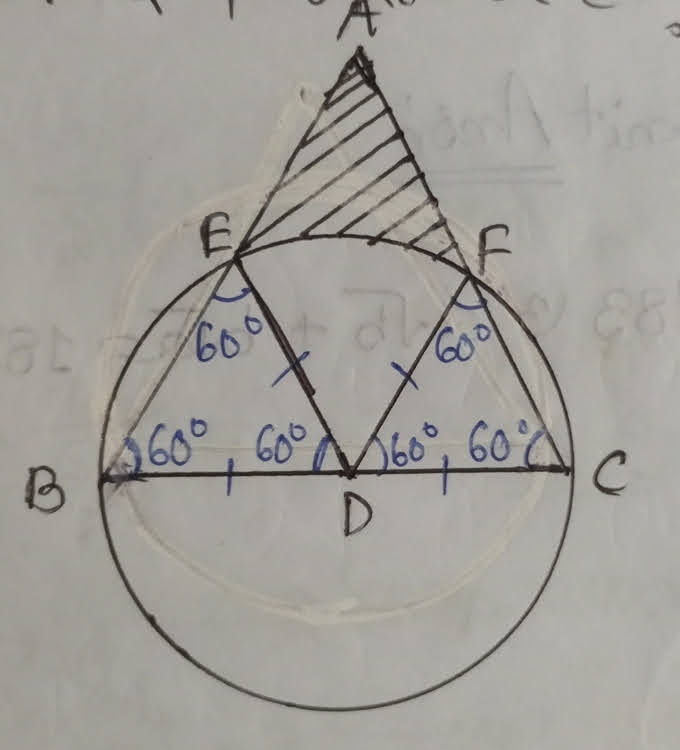
\includegraphics[scale = 0.25]{IMG_20230407_181844_861}\\
	\end{figure}
	
%58
	\item \textbengali{প্রমাণ কর যে, একটি বৃত্তের কোন একটি বহিস্থ বিন্দুগামী ওই বৃত্তের দুটি স্পর্শক বৃত্তে যে স্পর্শ জ্যা উৎপন্ন করে, সেই স্পর্শ জ্যাটিকে ওই বৃত্তের কেন্দ্র ও সেই বহিস্থ বিন্দুগামী সরলরেখাংশ লম্বভাবে সমদ্বিখণ্ডিত করে।}
	 
%59
	\item $O$ \textbengali{কেন্দ্রীয় বৃত্তের} $AB$ \textbengali{একটি জ্যা।} $A$ \textbengali{ও} $B$ \textbengali{বিন্দুতে অঙ্কিত স্পর্শকদ্বয় পরস্পরকে} $P$ \textbengali{বিন্দুতে ছেদ করে।} $P$ \textbengali{বিন্দুগামী একটি বৃত্ত} $AB$ \textbengali{জ্যাকে} $A$ \textbengali{বিন্দুতে স্পর্শ করে। বর্ধিত} $OA$ \textbengali{দ্বিতীয় বৃত্তকে} $D$ \textbengali{বিন্দুতে ছেদ করে। প্রমাণ কর যে, } $OA = AD.$
	
%60
	\item $ABC$ \textbengali{ও} $DEF$ \textbengali{দুটি সদৃশকোণী  ত্রিভুজ।}  \textbengali{প্রমাণ কর যে, } $$\dfrac{\bigtriangleup ABC}{\bigtriangleup DEF} = \dfrac{BC^2}{EF^2} = \dfrac{AB^2}{DE^2} = \dfrac{AC^2}{DF^2}.$$
	
%61
	\item  Given $x:y:z = 3:4:5$. Find $x$, $y$, $z$.
	\begin{figure}[h]
	\centering
	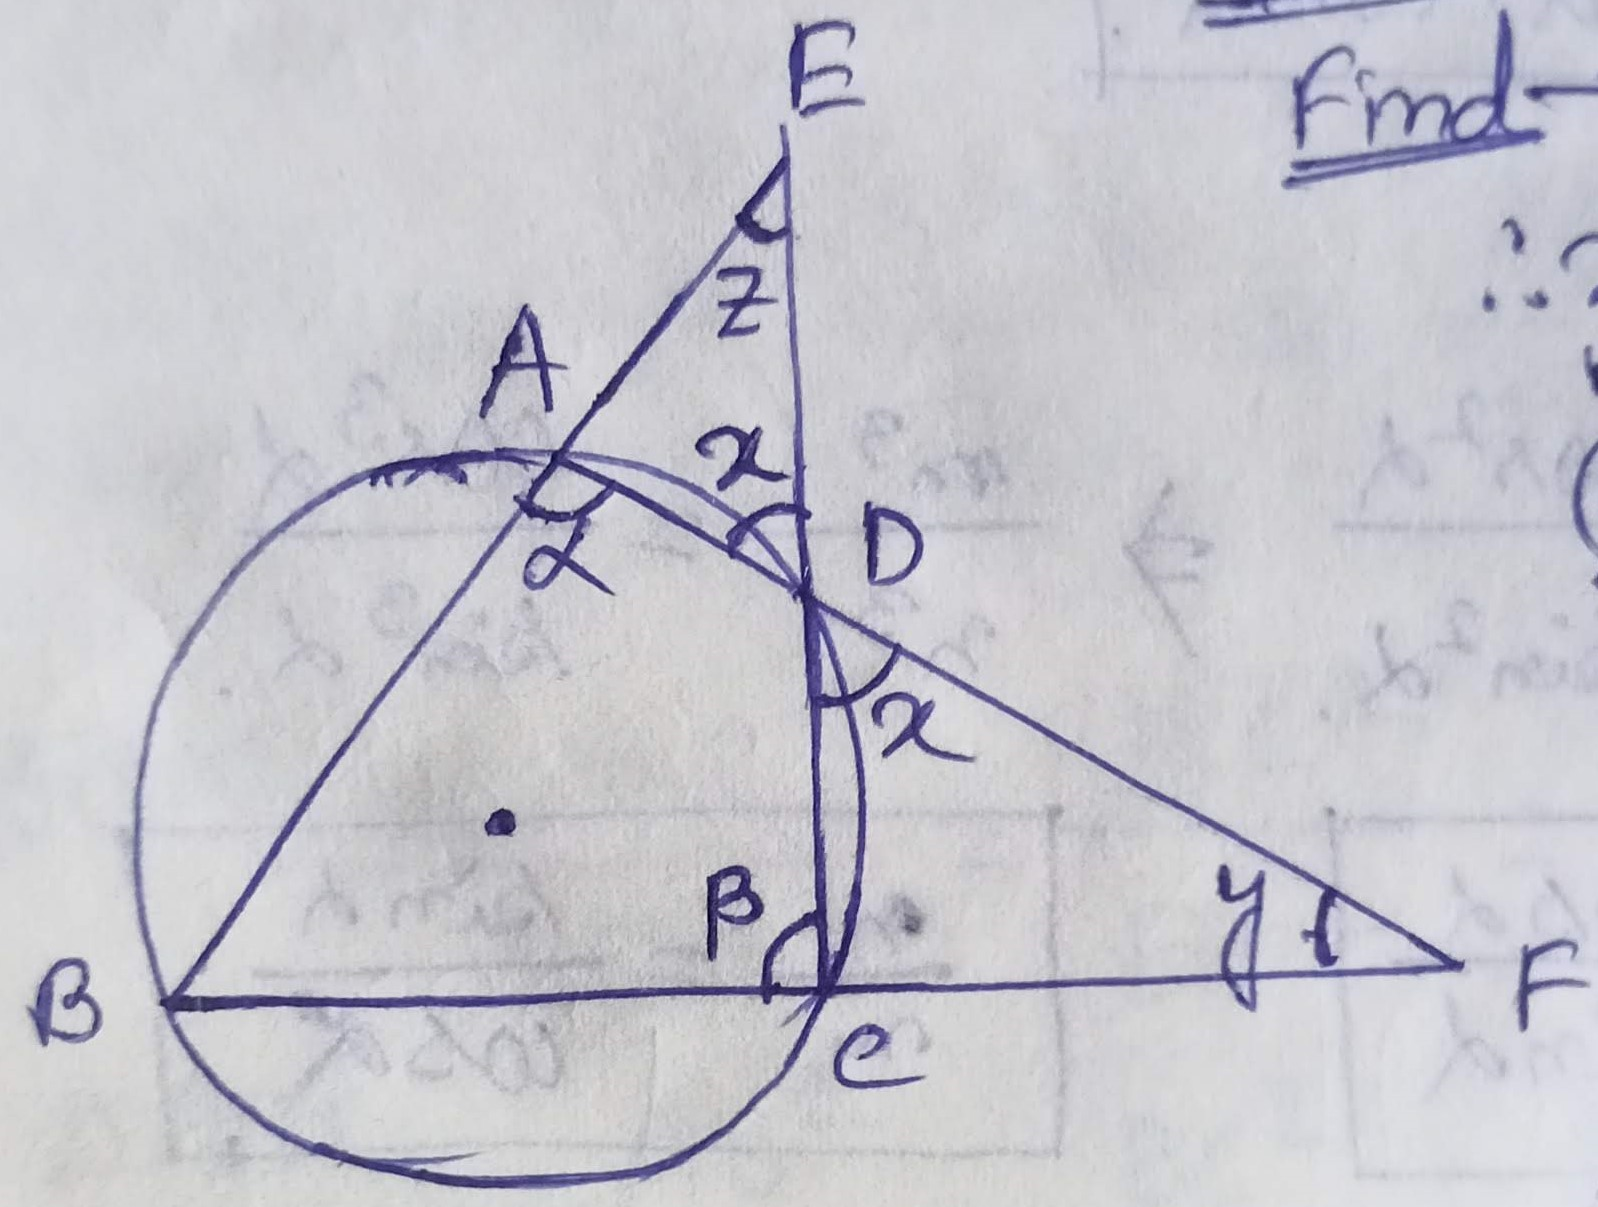
\includegraphics[scale = 0.1]{IMG_20230723_153249_398}\\
	\end{figure}

%62
	\item \textbengali{কোনো বৃত্তস্থ চতুর্ভুজের বিপরীত বাহুগুলি বর্ধিত করার ফলে যে দুটি কোণ উৎপন্ন হয় তাদের অন্তঃসমদ্বিখণ্ডকদ্বয়ের মধ্যবর্তী কোণের মান কত ?}

%63
	\item \textbengali{প্রমাণ কর যে, কোনো ট্রাপিজিয়ামের সমান্তরাল বাহুদ্বয়ের সঙ্গে সমান্তরালভাবে অঙ্কিত একটি সরলরেখা তির্যক বাহুদ্বয়কে বা তাদের বর্ধিত অংশকে সমানুপাতে বিভক্ত করে।} 
	
%64
	\item \textbengali{দুটি বৃত্ত পরস্পরকে ছেদ করে একটি সাধারণ জ্যা উৎপন্ন করেছে।  সাধারণ জ্যায়ের যেকোনো একটি প্রান্তবিন্দুতে অঙ্কিত দুটি সরলরেখার প্রত্যেকটি বৃত্তদ্বয়কে যথাক্রমে} $A$, $B$ \textbengali{ও} $C$, $D$ \textbengali{বিন্দুতে ছেদ করেছে।} $AB$ \textbengali{ও} $CD$ \textbengali{সরলরেখাংশদ্বয় সাধারণ জ্যাটির সঙ্গে সমান কোণে নত। প্রমাণ কর যে, }$AB = CD$.
	
%65
	\item \textbengali{প্রমাণ কর যে, দুটি পরস্পরছেদী বৃত্তের ছেদবিন্দুদ্বয়ের যেকোনো একটি বিন্দুগামী সকল সরলরেখাগুলির মধ্যে যে সরলরেখাটি বৃত্তদ্বয়ের কেন্দ্রের সংযোজক সরলরেখাংশের সমান্তরাল সেটিই ক্ষুদ্রতম সরলরেখা।}
	
%66
	\item Two circles of radius $a$ and $b$ touch each other externally and they also touch a line. A circle of radius $c$ is inscribed in the region in between the circles and the line to touch the both of the circles. Show that, $\dfrac{1}{\sqrt{c}} = \dfrac{1}{\sqrt{a}} + \dfrac{1}{\sqrt{b}}$.
	
%67
	\item Two circles $C_1$ and $C_2$ of radii $a$ and $b$ touch each other externally and they both touch a unit circle $C$ internally. A circle $C_3$ of radius $r$ is inscribed to touch the circles $C_1$, $C_2$ externally and $C_3$ internally. Show that, $r = \dfrac{ab}{1-ab}$.
	
%68
	\item \textbengali{দুটি বৃত্ত পরস্পরকে} $P$ \textbengali{বিন্দুতে অন্তঃস্পর্শ করে।} $ABCD$ \textbengali{সরলরেখাংশ বহিঃস্থ বৃত্তকে} $A$, $D$ \textbengali{ও অন্তঃস্থ বৃত্তকে} $C$ \textbengali{ও} $B$ \textbengali{বিন্তুতে ছেদ করে।} $\angle APB = 20^{\circ}$ \textbengali{হলে} $\angle CPD = $ \textbengali{কত ?}
	
%69
	\item $ABCD$ \textbengali{রম্বসের} $C$ \textbengali{বিন্দুগামী একটি সরলরেখা} $AB$ \textbengali{ও বর্ধিত} $DA$ \textbengali{কে যথাক্রমে} $P$ \textbengali{ও} $Q$ \textbengali{বিন্দুতে ছেদ করে। প্রমাণ কর যে, }
	\begin{enumerate}[(i)]
		\item $\bigtriangleup APQ$, $\bigtriangleup BPC$, $\bigtriangleup DCQ$ \textbengali{প্রত্যেকে পরস্পরের সঙ্গে সদৃশকোণী।}
		\item $PB : DQ = AP^2 : AQ^2 $.
	\end{enumerate}
		

%70
	\item $O$ \textbengali{কেন্দ্রীয় একটি বৃত্তে ত্রিভুজ} $ABC$ \textbengali{অন্তর্লিখিত। বৃত্তের ওপর অবস্থিত } $X$ \textbengali{বিন্দু থেকে} $AB$ \textbengali{বাহুর ওপর} $XP$ \textbengali{লম্ব এবং} $AC$ \textbengali{বাহুর ওপর} $XQ$ \textbengali{লম্ব।} $BK$ \textbengali{বৃত্তটির একটি ব্যাস হলে প্রমাণ কর যে, } $PQ : BC = AX : 2R$  ,\textbengali{যেখানে বৃত্তটির \\ ব্যাসার্ধ = } $R$.
	
%71
	\item In an acute triangle $ABC$; points $D$, $E$, $F$ are located on the sides $BC$, $CA$, $AB$ respectively such that $$\dfrac{CD}{CE} = \dfrac{CA}{CB}, \dfrac{AE}{AF} = \dfrac{AB}{AC}, \dfrac{BF}{BD} = \dfrac{BC}{BA}.$$ Prove that, $AD$, $BE$, $CF$ are altitudes of $ABC$. [RMO 2002]
	
%72
	\item Let $ABC$ be a triangle in which $AB=AC$ and $\angle CAB = 90^{\circ}$. Suppose $M$ and $N$ are points on the hypotenuse $BC$ such that $BM^2 + CN^2 = MN^2.$ Prove that $\angle MAN = 45^{\circ}.$ [RMO 2003]
	
%73
	\item Let $ABC$ be a triangle in which $AB = AC$ and let $I$ be its in-centre. Suppose $BC = AB + AI$. Find $\angle BAC .$ [RMO 2009]
	
%74
	\item Let $AB$ be a triangle and let $BB_1$, $CC_1$ be respectively the bisectors of $\angle B$, $\angle C$ with $B_1$ on $AC$ and $C_1$ on $AB$. Let $E$, $F$ be the feet of perpendiculars drawn from $A$ onto $BB_1$, $CC_1$ respectively. Suppose $D$ is the point at which the incircle of $ABC$ touches $AB$. Prove that, $AD = EF$.
	
%75
	\item Consider in the plane a circle $\Gamma$ with center $O$ and a line $l$ not intersecting circle $\Gamma$. Prove that there is a unique point $Q$ on the perpendicular drawn from $O$ to the line $l$, such that for any point $P$ on the line $l$, $PQ$ represents the length of the tangent from $P$ to the circle $\Gamma$. [RMO 2004]
	
%76
	\item Euler's Theorem : \textbengali{কোনো ত্রিভুজের পরিব্যাসারধ} $R$, \textbengali{অন্তঃব্যাসার্ধ} $r$, \textbengali{পরিকেন্দ্র} $S$ \textbengali{ও অন্তঃকেন্দ্র} $I$ \textbengali{হলে প্রমাণ কর যে, } $SI^2 = R^2 - 2Rr$.
	
%77
	\item Euler's Theorem : \textbengali{কোনো ত্রিভুজের পরিব্যাসারধ} $R$, \textbengali{বহিঃব্যাসার্ধ} $r_1$, \textbengali{পরিকেন্দ্র} $S$ \textbengali{ও বহিঃকেন্দ্র} $I_1$ \textbengali{হলে প্রমাণ কর যে, } $S{I_1}^2 = R^2 + 2Rr_1$.
	
%78
	\item $\bigtriangleup ABC$ \textbengali{এর} $S$ \textbengali{পরিকেন্দ্র,} $I$ \textbengali{অন্তঃকেন্দ্র,} $O$ \textbengali{লম্ববিন্দু হলে প্রমাণ কর যে,} $\angle SAI = \angle IAO.$
	
%79
	\item $\bigtriangleup ABC$ \textbengali{এর} $\angle BAC = 90^{\circ}$, $AD \perp BC$. $\angle ABC$ \textbengali{ও} $\angle CAD$ \textbengali{কোণের  অন্তঃসমদ্বিখণ্ডকদ্বয় যথাক্রমে} $BE$ \textbengali{ও} $AF$. $BE$, $AD$ \textbengali{কে} $E$ \textbengali{বিন্দুতে ও} $AF$, $CD$ \textbengali{কে} $F$ \textbengali{বিন্দুতে ছেদ করে। প্রমাণ কর যে,} $EF \parallel AC.$
	
%80
	\item $\bigtriangleup ABC$ \textbengali{সমদ্বিবাহু যার} $AC=BC$. $BP \perp AC$, $PN \perp BC$. \textbengali{প্রমাণ কর যে,} $AB^2 = AN^2 + PN^2$.
	
%81
	\item $O$ \textbengali{কেন্দ্রীয় বৃত্তের} $AB$ \textbengali{একটি ব্যাস।} $AB$ \textbengali{ব্যাসের একই পাশে} $P$ \textbengali{ও} $Q$ \textbengali{দুটি এমন বিন্দু যে} $Q$, $AP$ \textbengali{চাপের মধ্যে ও} $P$, $BQ$ \textbengali{চাপের মধ্যে অবস্থিত। বর্ধিত} $AQ$ \textbengali{ও বর্ধিত} $BP$ \textbengali{পরস্পরকে} $Y$ \textbengali{বিন্দুতে এবং} $AP$ \textbengali{ও} $BQ$ \textbengali{পরস্পরকে} $X$ \textbengali{বিন্দুতে ছেদ করে। প্রমাণ কর যে,} $P$ \textbengali{ও} $Q$ \textbengali{বিন্দুতে অঙ্কিত স্পর্শকদ্বয়} $XY$ \textbengali{এর মধ্যবিন্দুগামী।}
	
%82
	\item \textbengali{প্রমাণ কর যে, কোনো ত্রিভুজের পরিব্যাসার্ধ তার বাহুগুলির মধ্যবিন্দু গুলির সংযোজক সরলরেখাংশগুলি দ্বারা গঠিত ত্রিভুজের পরিব্যাসার্ধের দ্বিগুণ।}
	
%83
	\item $AB$ \textbengali{সরলরেখাংশের} $A$ \textbengali{ও} $B$ \textbengali{বিন্দুতে যথাক্রমে} $RA$ \textbengali{ও} $QB$ \textbengali{লম্ব।} $AQ$ \textbengali{ও} $BR$ \textbengali{পরস্পরকে} $O$ \textbengali{বিন্দুতে ছেদ করে।} $OT \perp AB$. \textbengali{প্রমাণ কর যে,} $OT$, $\angle QTR$ \textbengali{কে সমদ্বিখণ্ডিত করে।}
	
%84
	\item $ABCD$ \textbengali{ট্রাপিজিয়ামের} $AD \parallel BC$. \textbengali{কর্ণদ্বয়} $AC$ \textbengali{ও} $BD$ \textbengali{এর ছেদবিন্দু} $F$. $F$ \textbengali{বিন্দুগামী} $AD$ \textbengali{এর সমান্তরাল সরলরেখা} $AB$ \textbengali{ও} $CD$ \textbengali{কে যথাক্রমে} $E$ \textbengali{ও} $G$ \textbengali{বিন্দুতে ছেদ করেছে। প্রমাণ কর যে,} $EF = FG$.
	
%85
	\item $ABCD$ \textbengali{একটি সামান্তরিক। প্রমাণ কর যে,} $AB^2 + BC^2 + CA^2 + AD^2 = AC^2 + BD^2$.
	
%86
	\item $ABCD$ \textbengali{বর্গক্ষেত্রের} $AB$, $BC$, $CD$ \textbengali{ও} $DA$ \textbengali{বাহুগুলির মধ্যবিন্দুগুলি হল যথাক্রমে} $E$, $F$, $G$ \textbengali{ও} $H$. $AF$, $CE$ \textbengali{পরস্পরকে} $P$ \textbengali{এবং} $AG$ \textbengali{ও} $CH$ \textbengali{পরস্পরকে} $Q$ \textbengali{বিন্দুতে ছেদ করলে প্রমাণ কর যে,} $APCQ$ \textbengali{একটি রম্বস।}
	
%87
	\item \textbf{Morley's Theorem} : The points of intersection of the adjacent trisectors of the angles of any triangle form the vertices of an equilateral triangle.
	
%88
	\item \textbengali{একটি বৃত্তে} $AB$ \textbengali{ও} $CD$ \textbengali{হল দুটি পরস্পর লম্বভাবে অবস্থিত ব্যাস। বৃত্তের ওপর অবস্থিত} $P$ \textbengali{একটি যেকোনো বিন্দু। প্রমাণ কর যে,} $4 \bigtriangleup PCD = PA^2 \sim PB^2$.
	
%89
	\item $ABCD$ \textbengali{চতুর্ভুজের} $AC$ \textbengali{ও} $BD$ \textbengali{কর্ণদ্বয় পরস্পরকে} $O$ \textbengali{বিন্দুতে ছেদ করে। একই সমতলে অবস্থিত একটি} $\bigtriangleup PQR$ \textbengali{এর} $PQ$ \textbengali{ও} $PR$ \textbengali{বাহুদ্বয় যথাক্রমে} $BD$ \textbengali{ও} $AC$ \textbengali{এর সঙ্গে সমান ও সমান্তরাল। প্রমাণ কর যে,} $ABCD$ \textbengali{চতুর্ভুজের ক্ষেত্রফল} $=$ $\bigtriangleup PQR$ \textbengali{এর ক্ষেত্রফল।}
	
%90
	\item $ABCD$ \textbengali{চতুর্ভুজের} $AB$ \textbengali{ও} $CD$ \textbengali{বাহুর ওপর যথাক্রমে অবস্থিত} $E$,$F$ \textbengali{এবং} $G$,$H$ \textbengali{বিন্দুগুলি বাহুদ্বয়কে সমত্রিখণ্ডিত করে। প্রমাণ কর যে,} $EFGH$ \textbengali{চতুর্ভুজের ক্ষেত্রফল} $= \dfrac{1}{2}$ $\big( AEHD$ \textbengali{চতুর্ভুজের ক্ষেত্রফল} $+$ $BCGF$ \textbengali{চতুর্ভুজের ক্ষেত্রফল} $\big)$.
	
%91
	\item $P$ \& $Q$ are two points on $BC$ of $\bigtriangleup ABC$ such that $BP = QC$. If the bisector of $\angle B$ meets $AP$, $AQ$ \& $AC$ respectively at $X$, $Y$ and $Z$, show that, $\dfrac{PX}{AX} + \dfrac{QY}{AY} = \dfrac{CZ}{AZ}$.
	
%92
	\item $M$ \textbengali{ও} $N$ \textbengali{কেন্দ্রীয় দুটি বৃত্ত পরস্পরকে} $A$ \textbengali{ও} $B$ \textbengali{বিন্দুতে ছেদ করেছে।} $PQ$ \textbengali{ও} $RS$ \textbengali{হল বৃত্তদ্বয়ের সরল সাধারণ স্পর্শকদ্বয়।} \textbengali{বর্ধিত} $BA$, $PQ$ \textbengali{কে} $D$ \textbengali{বিন্দুতে ছেদ করে। প্রমাণ কর যে, } $PQ^2 + AB^2 = CD^2$.
	
%93
	\item Let $\Gamma$ be a circle with center $O$ and $P$ be any point on its plane. Then show that, the power of $P$ w.r.t. $\Gamma$ is $OP^2 - R^2$ where $R$ is the radius of $\Gamma$.
	
%94
	\item $O$ \textbengali{কেন্দ্রীয় একটি বৃত্তে} $AB$ \textbengali{ও} $BC$ \textbengali{দুটি জ্যা।} $AB$ \textbengali{এর ওপর অবস্থিত} $D$ \textbengali{এমন একটি বিন্দু যাতে} $\angle DCB = 40^{\circ}$ \textbengali{হয়।} $OC$ \textbengali{ব্যাসার্ধটি} $\angle DBC$ \textbengali{কোণের সমদ্বিখণ্ডক।} $\angle ABC = 30^{\circ}$. $\angle CDO = $ \textbengali{কত ?}
	
%95
	\item $ABCD$ \textbengali{সামান্তরিকের} $AB$ \textbengali{বাহুর সমান্তরাল একটি সরলরেখা} $QP$. $AP$, $BQ$ \textbengali{পরস্পরকে} $R$ \textbengali{এবং} $CQ$, $DP$ \textbengali{পরস্পরকে} $S$ \textbengali{বিন্দুতে ছেদ করেছে। প্রমাণ কর যে,} $RS \parallel AD$.
	
%96
	\item $ABCD$ \textbengali{একটি বৃত্তস্থ চতুর্ভুজ যার} $AB > CD$, $AD > BC$. $P$ \textbengali{এবং} $Q$ \textbengali{হল যথাক্রমে} $AB$ \textbengali{ও} $AD$ \textbengali{এর ওপর অবস্থিত এমন দুটি বিন্দু যে} $BP = CD$ \textbengali{ও} $DQ = BC$ \textbengali{হয়।} $M$, $PQ$ \textbengali{এর মধ্যবিন্দু। প্রমাণ কর যে,} $\angle BMD = 90^{\circ}$.
	
%97
	\item \textbengali{জ্যামিতিক উপায়ে প্রমাণ কর যে,} $3 < \pi < 4$.
	
%98
	\item $ABC$ is an isosceles triangle where $\angle A = 20^{\circ}$, $AB = AC$. $D$ \& $E$ are points on $AB$ \& $AC$ respectively such that $\angle BCD = 60^{\circ}$ \& $\angle CBE = 70^{\circ}$. Find $\angle BED$.
	
	
%99
	\item $\bigtriangleup ABC$ \textbengali{এর তিনটি মধ্যমা} $AD$, $BE$, $CF$ \textbengali{হলে দেখাও যে,} $$3(AB^2 + BC^2 + CA^2) = 4(AD^2 + BE^2 + CF^2)$$.
	
%100
	\item \textbengali{কোনো বৃত্তের} $AC$ \textbengali{ও} $BD$ \textbengali{দুটি জ্যা পরস্পরকে} $O$ \textbengali{বিন্দুতে ছেদ করেছে।} $A$ \textbengali{ও} $B$ \textbengali{বিন্দুতে অঙ্কিত স্পর্শক দুটি পরস্পরকে} $P$ \textbengali{বিন্দুতে এবং} $C$ \textbengali{ও} $D$ \textbengali{বিন্দুতে অঙ্কিত স্পর্শক দুটি পরস্পরকে} $Q$ \textbengali{বিন্দুতে ছেদ করলে প্রমাণ কর যে,} $\angle P + \angle Q = 2 \angle BOC$.
	

%101
	\item $\bigtriangleup ABC$ \textbengali{এর} $\angle C = 90^{\circ}$. $\bigtriangleup ABC$ \textbengali{এর অন্তঃবৃত্ত} $AB$, $BC$ \textbengali{ও} $CA$ \textbengali{কে যথাক্রমে} $F$, $D$, $E$ \textbengali{বিন্দুতে ছেদ করে।} $AD$ \textbengali{অন্তঃবৃত্তকে} $P$ \textbengali{বিন্দুতে ছেদ করে।} $\angle BPC = 90^{\circ}.$ \textbengali{দেখাও যে,} $AE + AP = PD$.
	
%102
	\item Let $ABC$ be a triangle, $AD$ the altitude through $A$ and $AK$ the circumdiameter through $A$. Then show that, $\angle DAK = \angle B - \angle C$. Further show that, the angular bisector $AX$ of $\angle A$ bisects $\angle DAK$.
	
%103
	\item If the internal bisector of $\angle A$ of $\bigtriangleup ABC$ meets $BC$ at $X$, then show that the difference between $\angle AXB$ and $\angle AXC$ is the same as the difference between $\angle B$ and $\angle C$.
	
%104
	\item If $m_a$, $m_b$, $m_c$ are the lengths of the medians of $\bigtriangleup ABC$ through $A$, $B$, $C$ then prove that,
		\begin{enumerate}[(i)]
			\item $2m_a^2 = b^2 + c^2 - \dfrac{a^2}{2}$
			
			\item $2m_b^2 = c^2 + a^2 - \dfrac{b^2}{2}$
		
			\item $2m_c^2 = a^2 + b^2 - \dfrac{c^2}{2}$
		\end{enumerate}
		
%105
	\item Prove that, $m_a ^2 + m_b^2 + m_c^2 = \dfrac{3}{4}\left( a^2 + b^2 + c^2 \right)$.
	
%106
	\item Prove that, $GA^2 + GB^2 + GC^2 = \dfrac{1}{3} \left(a^2 + b^2 + c^2 \right)$ where $G$ is the centroid of any triangle $\bigtriangleup ABC$.
	
%107
	\item If $P$ is any point in the plane of $\bigtriangleup ABC$, then $PA^2 + PB^2 + PC^2 = GA^2 + GB^2 + GC^2 + 3PG^2$, where $G$ is the centroid of $\bigtriangleup ABC$.
	
%108
	\item If $G$ is the centroid, $R$ is the circumradius and $S$ is the circumcenter of $\bigtriangleup ABC$, show that, $$SG^2 = R^2 - \dfrac{1}{9} \left( a^2 + b^2 + c^2 \right).$$
	
%109
	\item The incenter $I$ and the excenter $I_a$ opposite to $A$ divide the bisector $AU$ harmonically, where $U$ is the point of intersection of the internal bisector of $\angle A$ and $BC$.
	
%110
	\item In a quadrilateral $ABCD$, the diagonals $AD$ and $BC$ meet at $O$. If it is given that $OA = OC$ and $OB = OD$, prove that, $BC = AD$ and that $\angle ACB = \angle CAD$.
	
%111
	\item In $\bigtriangleup ABC$, $\angle A = 60^{\circ}$, $AB > AC$, $O$ is the circumcenter and $H$ is the orthocenter. $M$, $N$ are points on the line segments $BH$ and $HF$ respectively such that $BM = CN$. Determine the value of $\dfrac{MH + NH}{OH}$.

%112
	\item In the acute angled triangle $ABC$, let $D$, $E$, $F$ be the feet of the altitudes through $A$, $B$, $C$ respectively and $H$ be the orthocenter of $\bigtriangleup ABC$. Prove that, $\dfrac{AH}{AD} + \dfrac{BH}{BE} + \dfrac{CH}{CF} = 2$.
	
%113
	\item \textbengali{কোনো সমকোণী ত্রিভুজের সমকোণ সংলগ্ন দুটি বাহুর একটি অপরটির দ্বিগুণ হলে প্রমাণ কর যে, উহার একটি কোণ} $30^{\circ}$ \textbengali{এর কম হবে।}
	
%114
	\item \textbengali{একটি সমকোণী ত্রিভুজের একটি সূক্ষ্মকোণ} $15^{\circ}$ \textbengali{ও অতিভুজ} $x$. \textbengali{ত্রিভুজটির ক্ষেত্রফল কত ?}
	
%115
	\item $P$ is a point on the minor arc $AB$ of the circumcircle of the square $ABC$. Prove that, $\dfrac{PA + PC}{PB+PD} = \dfrac{PD}{PC}$.
	
%116
	\item \textbf{[Langley's Problem]} $ABC$ \textbengali{সমদ্বিবাহু ত্রিভুজে} $\angle A = 20^{\circ}$, $AB = AC$. $AB$ \textbengali{ও} $AC$ \textbengali{এর ওপরে যথাক্রমে} $E$ \textbengali{ও} $D$ \textbengali{দুটি বিন্দু যাতে} $\angle DBE = 20^{\circ}$ \textbengali{ও} $\angle DCE = 30^{\circ}$ \textbengali{হয়।} $\angle BDE$ \textbengali{কত ?}
\end{enumerate}
		     
		  
		  
		  
		  
		  
		  
		  
		  
		  
		  
		  
		  
		  
		  
		  
		  
		  
		  
		  
		  
		  
		  
		  
		  
		  
		  
		     

\section{Miscellaneous}

\begin{enumerate}

%01

	\item \textbengali{যদি} 
	$ ab^2 + bc^2 + ca^2 = 0 $
	\textbengali{হয়  যখন} $ a,b,c \neq 0 $, 
	\textbengali{তবে} $ \left( \dfrac{a}{b} + \dfrac{b}{c} \right) + \left( \dfrac{b}{c} + \dfrac{c}{a} \right) + \left( \dfrac{c}{a} + \dfrac{a}{b} \right) +1 $
	\textbengali{এর মান কত?}

%02	
	\item $ 0<a<1 $ \textbengali{অর্থাৎ} $a$ \textbengali{সংখ্যাটি} $0$ \textbengali{ও} $1$ \textbengali{এর মধ্যে অবস্থিত হলে কোনটি সঠিক?}  \begin{enumerate}[A.]
	\item $a^2 < a$
	\item $a^2 = -a$
	\item $a^2 \geq a$
	\item $a^2 \geq 1$
	\end{enumerate}
	
%03
	\item \textbengali{শ্রীধর আচার্যের সূত্র}
	
%04
	\item If $ xyz = 1 $, show that, $ \left( x + \dfrac{1}{x} \right)^2 + \left( y + \dfrac{1}{y} \right)^2 + \left( z + \dfrac{1}{z} \right)^2 = 4 + \left( x + \dfrac{1}{x} \right) \left( y + \dfrac{1}{y} \right) \left( z + \dfrac{1}{z} \right) $.
	
%05
	\item $ \dfrac{a}{b-c} + \dfrac{b}{c-a} + \dfrac{c}{a-b} = 0 $ \textbengali{হলে} $ \dfrac{a}{(b-c)^2} + \dfrac{b}{(c-a)^2} + \dfrac{c}{(a-b)^2} $ \textbengali{এর মান নির্ণয় কর।}
	
%06
	\item $ a + b + c = 0 $ \textbengali{হলে} $ \left( \dfrac{a}{b-c} + \dfrac{b}{c-a} + \dfrac{c}{a-b} \right) \left( \dfrac{a-b}{c} + \dfrac{b-c}{a} + \dfrac{c-a}{b} \right) $ \textbengali{এর মান নির্ণয় কর।}
	
%07
	\item $ p(x+y)^2 = 5 $, $ q(x-y)^2 = 3 $ \textbengali{হলে} $ p^2(x+y)^2 + 4pqxy - q^2(x-y)^2  $ \textbengali{এর মান} $p$ \textbengali{ও} $q$ \textbengali{এর মাধ্যমে নির্ণয় কর।}
	
%08
	\item If $ x+y+z = 6 $, $ xy + yz + zx = 9 $, show that, $ \dfrac{1}{1-x} + \dfrac{1}{1-y} + \dfrac{1}{1-z} = 0 $.
	
%09
	\item $ \dfrac{x}{a-x} + \dfrac{y}{b-y} + \dfrac{z}{c-z} = 0 $ \textbengali{হলে} $ \dfrac{a}{a-x} + \dfrac{b}{b-y} + \dfrac{c}{c-z}  $ \textbengali{এর মান নির্ণয় কর।}
	
%10
	\item $k+l+m = 1$, $3(kl+lm+mk) = 1$ \textbengali{হলে} $k+l-2m$ \textbengali{এর মান কত?}
	
%11
	\item $x^2 + y^2 + z^2 = 6x - 8y - 25$ \textbengali{হলে} $x+y+z$ \textbengali{এর মান কত?}
	
%12
	\item $ \dfrac{x}{x-1} + \dfrac{y}{y-1} + \dfrac{z}{z-1} = 0 $ \textbengali{হলে} $ \dfrac{1}{1-x} + \dfrac{1}{1-y} + \dfrac{1}{1-z} $ \textbengali{এর মান কত?}
	
%13
	\item $ a+b+c = 1 = 3(ab+bc+ca) $ \textbengali{এবং} $abc = \dfrac{1}{27}$ \textbengali{হলে}
	\begin{enumerate}[(i)]
		\item $a$, $b$, $c$ \textbengali{এর মান কত?}
		\item $\dfrac{a}{b+c} + \dfrac{b}{c+a} + \dfrac{c}{a+b}$ \textbengali{এর মান কত?}
	\end{enumerate}
	
%14
	\item \textbengali{দেখাও যে,} $ \left( \dfrac{2}{x} - \dfrac{x}{2} \right) $ \textbengali{এর উৎপাদকগুলির সমষ্টি} $ \left( \dfrac{x}{2} + \dfrac{2}{x} \right) $.
	
%15
	\item If $ x + \dfrac{1}{x} = -1 $, find the value of $ x^{2017} + \dfrac{1}{x^{2017}} $.
	
%16
	\item $ p+q+r = 9 $, $ p^2 + q^2 + r^2 = 27 $, $ p^3 + q^3 + r^3 = 81 $, $ pqr $ = \textbengali{কত?}
	
%17
	\item If $ x+y+z = 0 $, show that, $ \left( \dfrac{yz}{2x^2 + yz} + \dfrac{zx}{2y^2 + zx} + \dfrac{xy}{2z^2 + xy} \right) = 1 $.
	
%18
	\item If $ x^3 + \dfrac{3}{x} = 4(a^3 + b^3) $ and $ 3x + \dfrac{1}{x^3} = 4(a^3 - b^3) $, show that $a^2 - b^2 = 1$.
	
	
%19
	\item If $ a+b+c = 0 $, prove that, $ a^7 + b^7 + c^7 = 7abc(ab+bc+ca)^2 $.	
	
%20
	\item Find the value of $\left( \sqrt{a-2\sqrt{a-1}} - \sqrt{a+2\sqrt{a-1}} \right)$ where $1 \leq a \leq 2$.
	
%21
	\item $-1 \leq \dfrac{3*x - 4}{7} \leq 5$ \textbengali{হলে} $x$ \textbengali{এর ক্ষুদ্রতম ও বৃহত্তম মান কত ?}
	
%22
	\item $ \left( x + \dfrac{1}{x} \right)^2 = 3 $ \textbengali{হলে} $ x^{36} + x^{30} + x^{26} + x^{20} + x^{18} + x^{12} + x^{6} + 1 $ = \textbengali{কত} ?
	
%23
	\item $ \left( x - \dfrac{1}{x} \right) = 1$ \textbengali{হলে} $ \dfrac{x^4 - \dfrac{1}{x^2}}{3x^2 + 5x - 3} $ = \textbengali{কত} ?
	
%24
	\item \textbengali{একটি বর্গক্ষেত্রের ভেতরে স্তম্ভ ও সারি বরাবর সমান তিনভাগ করা হল। তাদের প্রত্যেকটিতে} $1$ \textbengali{থেকে} $9$ \textbengali{পর্যন্ত পূর্ণসংখ্যার একটিকে এমনভাবে রাখা হল যাতে প্রত্যেক স্তম্ভ বরাবর, সারি বরাবর ও দুটি কর্ণ বরাবর সকল যোগফল সমান হয়। তবে প্রমাণ কর যে, একদম মাঝখানে রাখা সংখ্যাটি অবশ্যই} $5$ \textbengali{হবে।} 
	\begin{flushright}
		 MTRP 2014
	\end{flushright}
	
%25
	\item $a$ \textbengali{ও} $b$ \textbengali{দুটি ধনাত্মক বাস্তব সংখ্যা।} $ a\sqrt{a} + b\sqrt{b} = 183 $ \textbengali{ও} $ a\sqrt{b} + b\sqrt{a} =182 $. $ \dfrac{9}{5} \left( a+b \right) $ \textbengali{এর মান কত ?}
	 \begin{flushright}
	 	PRMO 2017
	\end{flushright}	  
	
	
%26
	\item $x$, $y$, $z$ \textbengali{বাস্তব ধনাত্মক সংখ্যা।} $x^2 + 4y^2 + 16z^2 = 48$ \textbengali{ও} $xy + 4yz + 2zx = 24$ \textbengali{হলে} $x^2 + y^2 + z^2 = $\textbengali{কত?}
	\begin{flushright}
	 	PRMO 2017
	\end{flushright}	
	
	
%27
	\item $\sqrt[3]{3} - \sqrt[3]{2}$ \textbengali{এর করণী নিরসক উৎপাদক কী?}
	
%28
	\item $\sqrt[3]{3} - \sqrt{2}$ \textbengali{এর করণী নিরসক উৎপাদক কী?}

%29 
	\item $\alpha$, $\beta$ are the two roots of the equation $x^2 -6x - 2 = 0$. If $a_n = \alpha^n - \beta^n$, \\ show that, $\dfrac{a_{10} - 2a_8}{2a_9} = 3.$
	
%30
	\item A root of the equation $4x^2 + 2x - 1 = 0$ is $\alpha$. $f(x) = 4x^3 - 3x + 1$. Find $2[f(\alpha) + \alpha].$
	
%31
	\item 20 \textbengali{টি চলকের মধ্যক (গড়)} 85. \textbengali{দুটি চলককে ভুল করে} 57 \textbengali{ও} 60 \textbengali{এর স্থানে} 75 \textbengali{ও} 70  \textbengali{নেওয়া হয়েছে। সঠিক মধ্যক কত ?}
	
%32
	\item 120 \textbengali{জন ছাত্রছাত্রীর গড় ওজন} 56 kg. \textbengali{ছাত্রদের গড় ওজন} 60 kg. \textbengali{ছাত্রীদের গড় ওজন} 50 kg. \textbengali{ছাত্র ও ছাত্রীদের সংখ্যা কী কী ?}
	
%33
	\item 3.2, 5.8, 7.9 \textbengali{ও} 4.5 \textbengali{চলকের পরিসংখ্যা যথাক্রমে} $x, x+2, x-3, x+6.$ \textbengali{গড়} 4.876 \textbengali{হলে} $x=$ \textbengali{কত ?}
	
%34
	\item If $x = \dfrac{\sqrt{a+2b} + \sqrt{a-2b}}{\sqrt{a+2b} - \sqrt{a-2b}}$, show that, $bx^2 -ax+b = 0.$
	
%35
	\item Find the value of $\dfrac{x+\sqrt{20}}{x-\sqrt{20}} + \dfrac{x+\sqrt{12}}{x-\sqrt{12}}$, given that, $x = \dfrac{4\sqrt{15}}{\sqrt{5} + \sqrt{3}}.$
	
%36
	\item \textbengali{সংখ্যাগুরুমান} (mode) \textbengali{নির্ণয়ের সূত্র।}
	
%37
	\item If $x + y + z = 4xyz$, show that, $\dfrac{x^2}{1 - 4x^2} + \dfrac{y^2}{1 - 4y^2} + \dfrac{z^2}{1 - 4z^2} = \dfrac{16x^2 y^2 z^2}{(1 - 4x^2) (1 - 4y^2) (1 - 4z^2)}.$

%38
	\item \textbengali{হীরকের দাম তার ওজনের বর্গের সঙ্গে সরলভেদে থাকে। সোনার ওপর হীরক বসিয়ে তৈরি তিনটি সমান ওজনের আংটির দাম যথাক্রমে} $x$ \textbengali{টাকা},  $y$ \textbengali{টাকা এবং} $z$ \textbengali{টাকা এবং আংটি তিনটিতে হীরকের ওজন যথাক্রমে} $3$, $4$ \textbengali{ও} $5$ \textbengali{ক্যারেট। দেখাও যে, এক ক্যারেট হীরকের দাম} $\left( \dfrac{x+z}{2} - y \right)$ \textbengali{টাকা।  (প্রতিটি আংটি তৈরির পারিশ্রমিক সমান)}

%39
	\item \textbengali{হীরকের মূল্য তার ওজনের বর্গের সঙ্গে সমানুপাতিক।} $8000$ \textbengali{টাকা মূল্যের একটি হীরকখণ্ড ভেঙে} $3$ \textbengali{টি খণ্ডে বিভক্ত করা হল। খণ্ড} $3$ \textbengali{টির ওজনের অনুপাত} $8:7:5$. \textbengali{ভাঙার ফলে কত ক্ষতি হল তা নির্ণয় কর।}
	
%40
	\item \textbengali{রিজার্ভ ব্যাংকের চলমান সিঁড়ি বেয়ে দুই ব্যাক্তি ওপরে উঠছিলেন। তাঁদের গতিবেগের অনুপাত} $1:2$. \textbengali{তাঁরা যথাক্রমে} $18$ \textbengali{টি ও } $27$ \textbengali{টি ধাপ অতিক্রম করে উপরে উঠলেন। চলমান সিঁড়িতে মত ধাপের সংখ্যা কত ?}

%41
	\item If $(a+b+c)x = (b+c-a)y = (c+a-b)z = (a+b-c)w$, then prove that, $x(yz + zw + yw) = yzw$.
	
%42
	\item If $x^2 - 2x + 4 = 0$, find out $x^6$ and $x$.
	
%43
	\item If $x^3 + \dfrac{1}{x^3} = 2$, find the value of $\left( x + \dfrac{1}{x} \right)$.
	
%44
	\item Show that, $\dfrac{5 + \sqrt{5}}{\sqrt{5 + 3\sqrt{5}}} = \sqrt[4]{20}$.
	
%45
	\item \textbengali{বর্গ বা বর্গমূল না করে প্রমাণ কর যে,} $\sqrt{5} + \sqrt{3} > \sqrt{6} + \sqrt{2}$.
	
%46
	\item $10\%$ \textbengali{হার সুদে} $8100$  \textbengali{টাকা ধার করে এক বছরের মধ্যে দুটি সমান কিস্তিতে শোধ করলে প্রতিটি কিস্তির পরিমাণ ক্কত ?}
	
%47
	\item \textbengali{একটি সন্দেশের বাক্সের দৈর্ঘ্য} $12$ $c.m.$, \textbengali{প্রস্থ} $10$ $c.m.$ \textbengali{ও উচ্চতা} $7$ $c.m.$ \textbengali{ওই বাক্সের মধ্যে} $2$ $c.m.$ \textbengali{বাহুবিশিষ্ট ঘনকাকার কতগুলি সন্দেশ রাখা যাবে ?}
	
%48
	\item \textbengali{একটি আয়তঘনাকার বাক্সের দৈর্ঘ্য} $6$ $c.m.$, \textbengali{প্রস্থ} $6$ $c.m.$ \textbengali{ও উচ্চতা} $5$ $c.m.$ \textbengali{ওই বাক্সের মধ্যে} $3$ $c.m.$ \textbengali{ব্যাসের কতগুলি গোলক রাখা যাবে ?}
	
%49
	\item $\left(x + \sqrt{x^2 - bc}\right) \left(y + \sqrt{y^2 - ca}\right) \left(z + \sqrt{z^2 - ab}\right) = \left(x - \sqrt{x^2 - bc}\right) \left(y - \sqrt{y^2 - ca}\right) \left(z - \sqrt{z^2 - ab}\right)$ \textbengali{হলে দেখাও যে প্রত্যেক পক্ষের মান} $\pm abc$ \textbengali{এর সমান।}
	
%50
	\item $x+\dfrac{1}{y} = y+\dfrac{1}{z} = z+\dfrac{1}{x}$ \textbengali{হলে দেখাও যে} $xyz = \pm 1$.

%51
	\item \textbengali{যদি} $a(b-c)x^2 + b(c-a)xy + c(a-b)y^2 = 0$ \textbengali{সমীকরণের বামপক্ষ একটি পূর্ণবর্গ রাশিমালা হয়, তবে প্রমাণ কর যে,} $\dfrac{1}{a} + \dfrac{1}{c} = \dfrac{2}{b}$.
	
%52
	\item $a^2 + b^2 + c^2 = x^2 + y^2 + z^2 = ax + by + cz$ \textbengali{হলে প্রমাণ কর যে,} $\dfrac{x}{a} = \dfrac{y}{b} = \dfrac{z}{c}$.
	
%53
	\item $a\left(x - y\right) + a^2 = b\left(y - z\right) + b^2 = c\left(z - x\right) + c^2$ \textbengali{হলে প্রমাণ কর যে, প্রত্যেকটির মান} $= \dfrac{a+b+c}{\frac{1}{a} + \frac{1}{b} + \frac{1}{c}}$.
	
%54
	\item If $2x = \sqrt{a} + \dfrac{1}{\sqrt{a}}$, show that, $\dfrac{\sqrt{x^2 - 1}}{x - \sqrt{x^2 - 1}} = \dfrac{1}{2} \left(a-1\right)$.
	
%55
	\item If $\dfrac{a}{b+c} + \dfrac{b}{c+a} + \dfrac{c}{a+b} = 1$, prove that, $\dfrac{a^2}{b+c} + \dfrac{b^2}{c+a} + \dfrac{c^2}{a+b} = 0$.
	
%56
	\item If $\dfrac{a^2}{b+c} + \dfrac{b^2}{c+a} + \dfrac{c^2}{a+b} = 0$, prove that, $\dfrac{a}{b+c} + \dfrac{b}{c+a} + \dfrac{c}{a+b} = 1$, provided $\left( a+b+c \right) \neq 0$.

%57
	\item If $a+b+c = 1$, $ab+bc+ca = \dfrac{1}{3}$, $abc = \dfrac{1}{27}$, prove that, $\dfrac{1}{a+bc} + \dfrac{1}{b+ca} + \dfrac{1}{c+ab} = \dfrac{27}{4}$.
	
%58
	\item If $\dfrac{by+cz}{b^2 + c^2} = \dfrac{cz+ax}{c^2+a^2} = \dfrac{ax+by}{a^2+b^2}$, prove that, $\dfrac{x}{a} = \dfrac{y}{b} = \dfrac{z}{c}$.
	
%59
	\item If $\dfrac{p}{a} + \dfrac{q}{b} + \dfrac{r}{c} = 1$ and $\dfrac{a}{p} + \dfrac{b}{q} + \dfrac{c}{r} = 0$, prove that, $\dfrac{p^2}{a^2} + \dfrac{q^2}{b^2} + \dfrac{r^2}{c^2} = 1$.
	
%60
	\item If $x\left( b-c \right) + y \left( c-a \right) + z\left( a-b \right) = 0$, show that, $\dfrac{bz-cy}{b-c} = \dfrac{cx-az}{c-a} = \dfrac{ay-bx}{a-b}$.
	
%61
	\item If $xy+yz+zx=1$, show that, $\left(1+x^2\right) \left(1+y^2\right)\left(1+z^2\right) = \{ \left(x+y\right)\left(y+z\right)\left(z+x\right) \}^2$.
	
%62
	\item If $x+y+z=1$, show that, $\dfrac{x+yz}{\left(x+y\right)\left(z+x\right)} + \dfrac{y+zx}{\left(y+z\right)\left(x+y\right)} + \dfrac{z+xy}{\left(z+x\right)\left(y+z\right)} = 3$.
	
%63
	\item If $a^2 - b^2 = b^2 - c^2 = c^2 - a^2$, prove that, $\dfrac{ab-c^2}{a-b} + \dfrac{bc-a^2}{b-c} + \dfrac{ca-b^2}{c-a} = 0$.
	
%64
	\item If $a+b+c=0$, prove that, $\dfrac{a^2}{2a^2 + bc} + \dfrac{b^2}{2b^2+ca} + \dfrac{c^2}{2c^2+ab} = 1$.

%65
	\item If $a+b+c=0$, prove that, $\dfrac{a^2+b^2+c^2}{a^3+b^3+c^3} + \dfrac{2}{3}\left( \dfrac{1}{a} + \dfrac{1}{b} + \dfrac{1}{c} \right) = 0$.
	
%66
	\item If $x = by + cz$, $y = cz + ax$, $z = ax + by$, prove that, $\dfrac{1}{1+a} + \dfrac{1}{1+b} + \dfrac{1}{1+c} = 2$.
	
%67
	\item If $ab+bc+ca = 0$, prove that, $\dfrac{1}{a^2 - bc} + \dfrac{1}{b^2 - ca} + \dfrac{1}{c^2 - ab} = 0$.
	
%68
	\item If $a^2 = by + cz$, $b^2 = cz + ax$, $c^2 = ax + by$, prove that, $\dfrac{x}{x+a} + \dfrac{y}{y+b} + \dfrac{z}{z+c} = 1$.
	
%69
	\item If $a+b+c=5$, $ab+bc+ca=8$, $abc=-7$, find the value of $\left( \dfrac{a^2}{b} + \dfrac{b^2}{a} \right) + \left( \dfrac{b^2}{c} + \dfrac{c^2}{b} \right) + \left( \dfrac{c^2}{a} + \dfrac{a^2}{c} \right)$.
	
%70
	\item If $\dfrac{a-b}{c} + \dfrac{b-c}{a} + \dfrac{c+a}{b} = 1$ and $a-b+c \neq 0$, show that, $\dfrac{1}{a} = \dfrac{1}{b} + \dfrac{1}{c}$.
	
%71
	\item If $\dfrac{b+c}{a} = \dfrac{c+a}{b} = \dfrac{a+b}{c}$, show that, $a+b+c=0$ or $a=b=c$.
	
%72
	\item If $\dfrac{1}{a} + \dfrac{1}{b} + \dfrac{1}{c} = \dfrac{1}{a+b+c}$, prove that, $\dfrac{1}{a^5} + \dfrac{1}{b^5} + \dfrac{1}{c^5} = \dfrac{1}{a^5 + b^5 + c^5} = \dfrac{1}{(a+b+c)^5}$.
	
%73
	\item If $a+b+c=0$, show that, $(a^2 + b^2 + c^2)^2 = 2(a^4 + b^4 + c^4)$.
	
%74
	\item If $x=a(b-c)$, $y=b(c-a)$, $z=c(a-b)$, show that, $\left( \dfrac{x}{a} \right)^3 + \left( \dfrac{y}{b} \right)^3 + \left( \dfrac{z}{c} \right)^3 = \dfrac{3xyz}{abc}$.
	
%75
	\item If $x=a^2-bc$, $y=b^2-ca$ and $z=c^2-ab$, prove that, $x^3+y^3+z^3-3xyz = \\ (a^3+b^3+c^3-3abc)^2$.

%76
	\item If $a+c=2b$, prove that, $a^2(b+c)+b^2(c+a)+c^2(a+b)=\dfrac{2}{9}(a+b+c)^3$.
	
%77
	\item If $x=b+c-a$, $y=c+a-b$, $z=a+b-c$, prove that, $x^3+y^3+z^3-3xyz = 4(a^3+b^3+c^3-3abc)$.

%78
	\item If $(a^2+b^2+c^2)(x^2+y^2+z^2) = (ax+by+cz)^2$, prove that, $\dfrac{x}{a} = \dfrac{y}{b} = \dfrac{z}{c}$.
	
%79
	\item \textbengali{একটি শূন্যগর্ভ জাহাজের ওজন এবং উহার অন্তর্গত মালপত্রের ওজন যথাক্রমে জাহাজের দৈর্ঘ্যের বর্গ ও ঘনের সাথে সরলভেদে আছে। যদি} $l_1$ \textbengali{দৈর্ঘ্যবিশিষ্ট জাহাজের মালপত্রসহ ওজন} $w_1$ \textbengali{এবং} $l_2$ \textbengali{ও} $l_3$ \textbengali{দৈর্ঘ্যবিশিষ্ট জাহাজের মালপত্রসহ ওজন} $w_2$ \textbengali{ও} $w_3$ \textbengali{হয় তবে প্রমাণ কর যে,} $$\dfrac{w_1}{{l_1}^2}\left( l_2 - l_3 \right) + \dfrac{w_2}{{l_2}^2}\left( l_3 - l_1 \right) + \dfrac{w_3}{{l_3}^2}\left( l_1 - l_1 \right) = 0$$.
	
%80
	\item If $a^{\frac{1}{3}} + b^{\frac{1}{3}} + c^{\frac{1}{3}} = 0$, prove that, $(a+b+c)^3 = 27abc$.
	
%81
	\item \textbengali{কোনো এক লীগের প্রতিযোগিতায় একটি দিনে যতগুলি খেলা হয় তা যুগ্মভাবে ওই দিন এবং বাকি দিনগুলির সঙ্গে ওই দিনের যোগফলের সহিত সমানুপাতে থাকে। যদি পরপর তিনদিন } $6$, $5$ \textbengali{এবং} $3$ \textbengali{টি খেলা হয়ে থাকে তবে কোন কোন দিন ওই খেলাগুলি হয়েছিল এবং প্রতিযোগিতাটি কত দিনের ছিল ?}
	
%82
	\item If $\dfrac{ay-bx}{c} = \dfrac{cx-az}{b} = \dfrac{bz-cy}{a}$, prove that, $\dfrac{x}{a} = \dfrac{y}{b} = \dfrac{z}{c}$.
	
%83
	\item If $a+b+c=0$, prove that, $a^5 + b^5 + c^5 = \dfrac{5}{6} (a^2 + b^2 + c^2) (a^3 + b^3 + c^3)$.
	
%84
	\item If $ax+by+cz=p$, $bx+cy+az=q$, $cx+ay+bz=r$, prove that, $p^3+q^3+r^3-3pqr = (a^3+b^3+c^3-3abc)(x^3+y^3+z^3-3xyz)$.
	
%85
	\item $x$, $y$, $z$ \textbengali{এমন তিনটি চলরাশি যে} $(y+z-x)$ \textbengali{এর মান ধ্রুবক এবং} $(z+x-y)(x+y-z)\propto yz$. \textbengali{প্রমাণ কর যে,} $(x+y+z) \propto yz$.
	
%86
	\item $(x+y) \propto z$ \textbengali{যখন} $y$ \textbengali{ধ্রুবক এবং} $(z+x) \propto y$ \textbengali{যখন} $z$ \textbengali{ধ্রুবক। প্রমাণ কর যে,} $(x+y+z) \propto yz$ \textbengali{যখন} $y$, $z$ \textbengali{উভয়েই চল।}
	
%87
	\item $x$ \textbengali{ও} $y$ \textbengali{দুটি ভিন্ন বাস্তব রাশি এবং} $x \propto y(x+y)$ \textbengali{ও} $y \propto x(x-y)$. \textbengali{প্রমাণ কর যে,} $(x^2 - y^2)$ \textbengali{এর মান} $x$ \textbengali{ও} $y$ \textbengali{এর ওপর নির্ভর করে না।}
	
%88
	\item $\dfrac{x}{y} \propto x-y $ \textbengali{ও} $\dfrac{y}{x} \propto x^2 + xy + y^2 $ \textbengali{হলে প্রমাণ কর যে,} $x^3 - y^3 = $ \textbengali{ধ্রুবক।}
	
%89
	\item If $u^2 + v^2 \propto x^2 + y^2$ and $uv \propto xy$, prove that, $u+v \propto x+y$ when $\dfrac{u}{v} + \dfrac{v}{y} = \dfrac{x}{y} + \dfrac{y}{x}$.
	
%90
	\item If $x \propto y$ and $y \propto z$ and $x=a$ when $y=b$, $z=c$ and $x = a'$ when $y = b'$, $z=c'$, prove that, $\dfrac{a^2 + b^2 + c^2}{aa' + bb' + cc'} = \dfrac{aa' + bb' + cc'}{(a')^2 + (b')^2 + (c')^2}$.
	
%91
	\item If $x \propto y + z$, $y \propto z + x$, $z \propto x + y$, and $a$, $b$, $c$ are three constants, prove that, $\dfrac{a}{a+1} + \dfrac{b}{b+1} + \dfrac{c}{c+1} = 1$, when $x+y+z \neq 0$.
	
%92
	\item If $ax^2 + 2hxy + by^2 \propto u^2$ and $lx+my \propto u$, prove that, $x \propto y$.
	
%93
	\item If $(x+y+z)(y+z-x)(z+x-y)(x+y-z) \propto x^2y^2$, prove that, $x^2 + y^2 = z^2$ or $x^2 + y^2 - z^2 \propto xy$.
	
%94
	\item $x$, $y$, $z$ are three variables such that $(x+y+z)$ is constant. $(x+z-y)(x+y-z) \propto yz$. Prove that, $(y+z-x) \propto yz$.
	
%95
	\item If $a+b+c=0$, prove that, $\dfrac{1}{a^2 + b^2 - c^2} + \dfrac{1}{b^2 + c^2 - a^2} + \dfrac{1}{c^2 + a^2 - b^2} = 0$.
	
%96
	\item If $(y+z) \propto x$ and $(z+x) \propto y$, prove that, $(x+y) \propto z$.



%97	
	\item Find the area of the shaded part in the following figure where $PQRS$ is a square and the length of each of the sides of the square is $x$. $P$, $Q$, $R$, $S$ respectively are the centers of ${\stackrel{{\mbox{$\Large{\frown}$}}}{SQ}}$, ${\stackrel{{\mbox{$\Large{\frown}$}}}{PR}}$, ${\stackrel{{\mbox{$\Large{\frown}$}}}{SQ}}$, ${\stackrel{{\mbox{$\Large{\frown}$}}}{PR}}$.
		
	\begin{figure}[H]
	\centering
	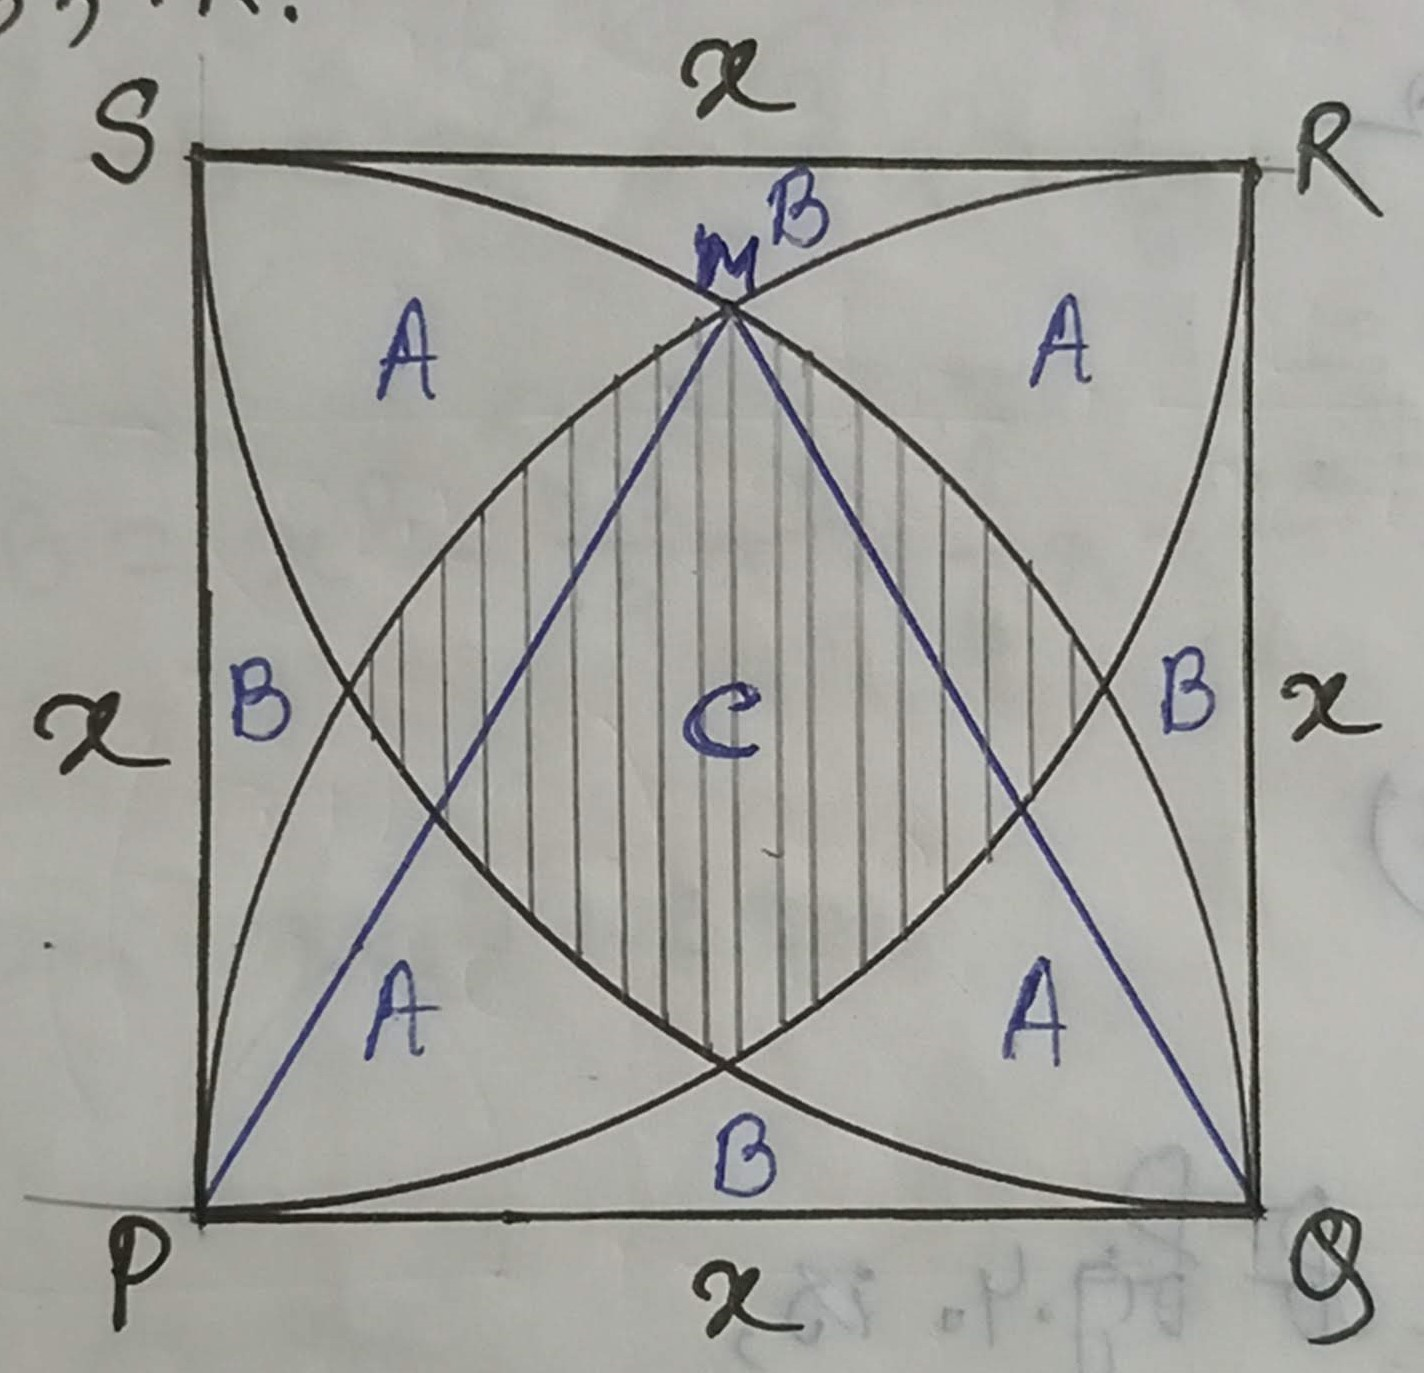
\includegraphics[scale = 0.15]{IMG_20230915_184133_844}\\
	\end{figure}


%98
	\item If $x+y : \sqrt{xy} = 4 : 1$, find $x:y$.
	
%99
	\item If $a : b = b : c$, show that, $a^2 b^2 c^2 \left( \dfrac{1}{a^3} + \dfrac{1}{b^3} + \dfrac{1}{c^3} \right) = a^3 + b^3 + c^3$.
	
%100
	\item If $a : b = b : c$, prove that, $\dfrac{abc(a+b+c)^3}{(ab+bc+ca)^3} = 1$.
	
%101
	\item If $3x - 4y \propto \sqrt{xy}$, prove that, $x^2 + y^2 \propto xy$.
	
%102
	\item If $\dfrac{x^2 - yz}{a} = \dfrac{y^2 - zx}{b} = \dfrac{z^2 - xy}{c}$, prove that, $x = y = z$.
	
%103
	\item \textbengali{কোনো ব্যক্তির পেনশনের পরিমাণ তার চাকুরী জীবনের বর্গমূলের সাথে সমানুপাতে থাকে। দুজন ব্যক্তির মধ্যে প্রথম ব্যক্তি দ্বিতীয় ব্যক্তি অপেক্ষা} $9$ \textbengali{বছর বেশি চাকরি করেন এবং} $500$ \textbengali{টাকা বেশি পেনশন পান। যদি প্রথম ব্যক্তি দ্বিতীয় ব্যক্তি অপেক্ষা} $4\dfrac{1}{4}$ \textbengali{বছর বেশি চাকরি করতেন তাহলে তাদের পেনশনের অনুপাত হত} $9:8$. \textbengali{তারা কত বছর চাকরি করেছেন? প্রত্যেকে কত টাকা পেনশন পেয়েছিলেন?}
	
%104
	\item If $a+b+c = 6$ and $ab+bc+ca = 9$, prove that, $\dfrac{1}{1-a} + \dfrac{1}{1-b} + \dfrac{1}{1-c} = 0$.
	
%105
	\item If $x^2 + y^2 + z^2 = xy + yz + zx$, prove that, $\dfrac{x^2}{yz} + \dfrac{y^2}{zx} + \dfrac{z^2}{xy} = 3$.
	
%106
	\item If $2s = a+b+c$, prove that, $(s-a)^3 + (s-b)^3 + 3(s-a)(s-b)c = c^3$.
	
%107
	\item If $2s = a+b+c$, prove that, $\dfrac{1}{s-a} + \dfrac{1}{s-b} + \dfrac{1}{s-c} - \dfrac{1}{s} = \dfrac{abc}{s(s-a)(s-b)(s-c)}$.
	
%108
	\item If $(a+b)^\frac{1}{3} + (b+c)^\frac{1}{3} + (c+a)^\frac{1}{3} = 0$, show that, $(a+b+c)^3 = 9(a^3 + b^3 + c^3)$.
	
%109
	\item If $\dfrac{1}{y} - \dfrac{1}{x} \propto \dfrac{1}{x-y}$, show that, $3x + y \propto \sqrt{xy}$.
	
%110
	\item If $2x^2 + 3y^2 \propto xy$, prove that, $9x^4 + 4y^4 \propto x^2y^2$.
	
%111
	\item If $2x + 3y \propto \sqrt{xy}$, prove that, $x \propto y$.
	
%112
	\item If $\dfrac{1}{x} + \dfrac{1}{y} \propto \dfrac{1}{x+y}$, prove that, $(x^2 + y^2) \propto xy$.
	
%113
	\item If $\dfrac{1}{x} - \dfrac{1}{y} \propto \dfrac{1}{x-y}$, prove that, $(x^2 + y^2) \propto xy$ and $x \propto y$.
	
%114
	\item If $\left( x^3 - \dfrac{1}{y^3} \right) \propto \left( x^3 + \dfrac{1}{y^3} \right)$, prove that, $x \propto \dfrac{1}{y}$.
	
%115
	\item $x \propto (y+z)$	, $y \propto (z+x)$, $z \propto (x+y)$ \textbengali{এবং} $a$, $b$, $c$ \textbengali{যথাক্রমে তিনটি ভেদের ধ্রুবক হলে দেখাও যে,} $ab+bc+ca+2abc = 1$.
	
%116
	\item If $(a+b+c) \propto (a+b-c)$ and $(a^2 + b^2 + c^2) \propto (a^2 + b^2 - c^2)$, prove that, $a \propto b$ and $b \propto c$.
	
%117
	\item \textbengali{যদি} $r_1$, $r_2$, $r_3$ \textbengali{ব্যাসার্ধবিশিষ্ট বৃত্তগুলির কেন্দ্রে যথাক্রমে} $l_1$, $l_2$, $l_3$ \textbengali{দৈর্ঘ্যের বৃত্তচাপগুলির দ্বারা উৎপন্ন কোণগুলির বৃত্তীয় মানগুলি} $a_1$, $a_2$, $a_3$ \textbengali{হয়, তবে প্রমাণ কর যে,} $\dfrac{1}{n} \left( a_1 r_1 + a_2 r_2 + a_3 r_3 \right)$ \textbengali{ব্যাসার্ধবিশিষ্ট কোনো বৃত্তের কেন্দ্রে} $\left( l_1 + l_2 + l_3 \right)$ \textbengali{দৈর্ঘ্যবিশিষ্ট কোনো বৃত্তচাপ যে কোণ উৎপন্ন করে তার বৃত্তীয় পরিমাপ হবে} $n$ \textbengali{রেডিয়ান।} 
	
%118
	\item \textbengali{যদি} $r_1$, $r_2$, $r_3$ \textbengali{ব্যাসার্ধবিশিষ্ট বৃত্তগুলির কেন্দ্রে যথাক্রমে} $l_1$, $l_2$, $l_3$ \textbengali{দৈর্ঘ্যের বৃত্তচাপগুলির দ্বারা উৎপন্ন কোণগুলির বৃত্তীয় মানগুলি} $\theta_1$, $\theta_2$, $\theta_3$ \textbengali{হয়, তবে প্রমাণ কর যে,} $\left( r_1 + r_2 + r_3 \right)$ \textbengali{ব্যাসার্ধবিশিষ্ট কোনো বৃত্তের কেন্দ্রে} $\left( l_1 + l_2 + l_3 \right)$ \textbengali{দৈর্ঘ্যবিশিষ্ট কোনো বৃত্তচাপ যে কোণ উৎপন্ন করে তার বৃত্তীয় পরিমাপ হবে} $\left( \dfrac{r_1 \theta_1 + r_2 \theta_2 + r_3 \theta_3}{r_1 + r_2 + r_3} \right)$ \textbengali{রেডিয়ান।} 
	
%119
	\item \textbengali{কোনো দ্বিঘাত সমীকরণ} $ax^2 + bx + c = 0 \, [a \neq 0]$ \textbengali{-এ} $b^2 = 9ac$ \textbengali{হলে সমীরণটির বীজদ্বয়ের মধ্যে সম্পর্ক কী?}
	
%120
	\item If $x = cy + bz$, $y = az + cx$, $z = bx + ay$, prove that, $\dfrac{x^2}{1-a^2} = \dfrac{y^2}{1-b^2} = \dfrac{z^2}{1-c^2}$.
	
%121
	\item If $x = bz + cy$, $y = cx + az$, $z = ay + bx$, prove that, $\dfrac{x}{\sqrt{1-a^2}} = \dfrac{y}{\sqrt{1-b^2}} = \dfrac{z}{\sqrt{1-c^2}}$.
	
%122
	\item If $x = \dfrac{1}{2} \left( \sqrt{\dfrac{a}{b}} - \sqrt{\dfrac{b}{a}}\right)$, find the value of $\dfrac{2a\sqrt{1+x^2}}{x+\sqrt{1+x^2}}$.
	
%123
	\item If $\sqrt{\left(x - \sqrt{a^2 - b^2}\right)^2 + y^2} + \sqrt{\left(x + \sqrt{a^2 - b^2}\right)^2 + y^2} = 2a$, prove that, $\dfrac{x^2}{a^2} + \dfrac{y^2}{b^2} = 1$.
	
%124
	\item If $y - mx = \sqrt{a^2 m^2 + b^2}$ and $x + my = \sqrt{a^2 + b^2 m^2}$, prove that, $x^2 + y^2 = a^2 + b^2$.
	
%125
	\item If $\dfrac{b}{x} + \dfrac{a}{y} \propto \dfrac{1}{ax+by}$, prove that, $x \propto y$.
	
%126
	\item If $x > y$, prove that, $\sqrt{y + \sqrt{2xy - x^2}} + \sqrt{y - \sqrt{2xy - x^2}} = \sqrt{2x}$.
	
%127
	\item \textbengali{একটি লম্ব বৃত্তাকার শঙ্কুর তির্যক উচ্চতা} $7 \, c.m.$ \textbengali{এবং সমগ্রতলের ক্ষেত্রফল} $147.84 \, sq. \, c.m.$ \textbengali{শঙ্কুটির ভূমির ব্যাসার্ধের দৈর্ঘ্য নির্ণয় কর।}
	
%128
	\item $1 \, c.m.$ \textbengali{ও} $6  \, c.m.$ \textbengali{দৈর্ঘ্যের ব্যাসার্ধ বিশিষ্ট দুটি নিরেট গোলককে গলিয়ে}  $1 \, c.m.$ \textbengali{পুরু ফাঁপা গোলকে পরিণত করা হলে, নতুন গোলকটির বাইরের বক্রতলের ক্ষেত্রফল কত ?}
	
%129
	\item \textbengali{কোনো মূলধনের} $2$ \textbengali{বছরের সুদ ও চক্রবৃদ্ধি সুদ যথাক্রমে} $8400$ \textbengali{টাকা ও} $8652$ \textbengali{টাকা হলে মূলধন ও বার্ষিক সুদের হার কত ?}
	
%130
	\item $a \propto \dfrac{1}{b}$ \textbengali{হলে প্রমাণ কর যে} $(a+b)$ \textbengali{এর মান ক্ষুদ্রতম যখন} $a = b$.
	
%131
	\item If $x = \dfrac{\sqrt{3}}{2}$, prove that, $\dfrac{\sqrt{1+x} + \sqrt{1-x}}{\sqrt{1+x} - \sqrt{1-x}} = \sqrt{3}$.
	
%132
	\item \textbengali{একটি হস্টেলের ব্যয় আংশিক ধ্রুবক ও আংশিক ওই হস্টেলবাসী লোকসংখ্যার সঙ্গে সরলভেদে আছে। লোকসংখ্যা} $120$ \textbengali{হলে ব্যয় হয়} $2000$ \textbengali{টাকা এবং লোকসংখ্যা} $100$ \textbengali{হলে ব্যয় হয়} $1700$ \textbengali{টাকা। ব্যয়} $1800$ \textbengali{টাকা হলে লোকসংখ্যা কত হবে ?}
	
%133
	\item \textbengali{মালগাড়ি সংযুক্ত না থাকলে একটি ইঞ্জিন ঘণ্টায়} $40$ \textbengali{মাইল বেগে যেতে পারে এবং এর সঙ্গে মালগাড়ি সংযুক্ত থাকলে এর গতিবেগ যে পরিমাণে হ্রাস পায় তা তার সঙ্গে সংযুক্ত মালগাড়ির সংখ্যার বর্গমূলের সঙ্গে সরলভেদে থাকে।} $16$ \textbengali{টি মালগাড়ি সংযুক্ত থাকলে তার গতিবেগ হয়} $20$ \textbengali{মাইল / ঘণ্টা।}
	\begin{enumerate}[(a)]
		\item \textbengali{ইঞ্জিনটি সবচেয়ে বেশি কতগুলি বগি নিয়ে চলতে সক্ষম থাকবে ?}
		\item \textbengali{সবচেয়ে কম কতগুলি বগি যোগ করলে চলতে অক্ষম হবে ?}
	
	\end{enumerate}
	
%134
	\item If $(x+z) :(y+z) = \left(\dfrac{x}{y} +2 \right) : \left( \dfrac{y}{x} + 2 \right)$, show that, $(x-z) : (y - z) = x^2 : y^2$.
	
%135
	\item \textbengali{কোনো পূর্ণবর্গ সংখ্যার ভাগ প্রক্রিয়ায় বর্গমূল করার সময়} $2$ \textbengali{গুণ করতে হয় কেন ?}
	
%136
	\item If $x^2 + y^2 + z^2 = 25$, $a^2 + b^2 + c^2 = 36$ and $ax + by + cz = 30$, find the value of $\dfrac{x+y+z}{a+b+c}$.
	
%137
	\item If $x = cy + bz$, $y = cx + az$ and $z = bx + ay$, prove that, $a^2 + b^2 + c^2 + 2abc = 1$.
	
%138
	\item If $x + y + xy = 5$, $y + z + yz = 7$ and $z + x + zx = 11$, prove that, $(1+x)^2(1+y)^2(1+z)^2 = 576$.
	
%139
	\item If $2x = a + \sqrt{\dfrac{4b^3 - a^3}{3a}}$ and $2y = a - \sqrt{\dfrac{4b^3 - a^3}{3a}}$, prove that, $x^3 + y^3 = b^3$.
	
%140
	\item If $\dfrac{a^2 - bc}{a^2 + bc} + \dfrac{b^2 - ca}{b^2 ++ ca} + \dfrac{c^2 - ab}{c^2 + ab} = 1$, prove that, $\dfrac{a^2}{a^2 + bc} + \dfrac{b^2}{b^2 + ca} + \dfrac{c^2}{c^2 + ab} = 2$.
	
%141
	\item \textbengali{সরল করঃ} $\dfrac{2 + \sqrt{3}}{\sqrt{2} + \sqrt{2 + \sqrt{3}}} + \dfrac{2 - \sqrt{3}}{\sqrt{2} - \sqrt{2 - \sqrt{3}}}$.
	
%142
	\item \textbengali{সরল করঃ} $\dfrac{\sqrt{26 - 15\sqrt{3}}}{5\sqrt{2} - \sqrt{38 + 5\sqrt{3}}}$.
	
%143
	\item Evaluate : $\dfrac{(4 + \sqrt{15})^\frac{3}{2} + (4 - \sqrt{15})^\frac{3}{2}}{(6 + \sqrt{35})^\frac{3}{2} + (6 - \sqrt{35})^\frac{3}{2}}$.
	
%144
	\item If $2x = \sqrt{\dfrac{p}{q}} - \sqrt{\dfrac{q}{p}}$, prove that, $\dfrac{2p\sqrt{x^2 + 1}}{x + \sqrt{x^2 + 1}} = p+q$.
	
%145
	\item If $x = y \sqrt{1 - z^2} + z \sqrt{1 - y^2}$, prove that, $(x + y + z)(y + z -x)(z + x - y)(x + y - z) = 4x^2 y^2 z^2$.
	
%146
	\item $x$ \textbengali{মুলদ রাশি}, $\sqrt{y}$ \textbengali{অমূলদ রাশি এবং} $\sqrt[3]{x + \sqrt{y}} = a + \sqrt{b}$ \textbengali{হলে দেখাও যে,} $\sqrt[3]{x - \sqrt{y}} = a - \sqrt{b}$.
	
%147
	\item If $x(x+1) = 1$, find the value of $(x-1)^3 - \dfrac{1}{(x-1)^3}$.
	
%148
	\item If $(x-7)(x-5) = 1$, find the value of $(x-5)^3 - \dfrac{1}{(x-5)^3}$.
	
%149
	\item If $a$, $b$, $c$ are real numbers, find the minimum and maximum values of $\dfrac{ab + bc + ca}{a^2 + b^2 + c^2}$.
	
%150
	\item If $\dfrac{a+b}{c} + \dfrac{b-c}{a} + \dfrac{c-a}{b} = 1$ and $(a+b-c) \neq 0$, prove that, $\dfrac{1}{a} + \dfrac{1}{c} = \dfrac{1}{b}$.
	
%151
	\item If $\dfrac{x+y}{x-y} = \dfrac{u}{v}$, prove that, $\dfrac{x^2 + xy}{xy - y^2} = \dfrac{u^2 - uv}{uv - v^2}$.
	
%152
	\item If $x+y+z = xyz$, prove that, $\dfrac{y+z}{1-yz} + \dfrac{z+x}{1-zx} + \dfrac{x+y}{1-xy} = \dfrac{y+z}{1-yz} \cdot \dfrac{z+x}{1-zx} \cdot \dfrac{x+y}{1-xy}$.
	
%153
	\item If $ab+bc+ca = abc$, prove that, $\dfrac{b+c}{bc(a-1)} + \dfrac{c+a}{ca(b-1)} + \dfrac{a+b}{ab(c-1)} = 1$.

%154
	\item \textbengali{যদি} $ax^2 + bx + c = 0$ \textbengali{সমীকরণের একটি বীজ অপরটির বর্গ হয়, তবে প্রমাণ কর যে,} $b^3 + ac^2 + a^2 c = 3abc$.
	
%155
	\item $ax^2 + bx + c = 0$ \textbengali{সমীকরণের বীজদ্বয়} $\alpha$ \textbengali{ও} $\beta$ \textbengali{হলে, প্রমাণ কর যে,} $a(x-\alpha) (x-\beta) = ax^2 + bx + c$.
	
%156
	\item $x^2 - px + q = 0$ \textbengali{সমীকরণের বীজদ্বয়ের সমষ্টি তাদের অন্তরের তিনগুণ হলে দেখাও যে,} $2p^2 = 9q$.
	
%157
	\item \textbengali{যদি} $x^2 - px + q = 0$ \textbengali{সমীকরণের বীজদ্বয়ের অন্তর} $1$ \textbengali{হয়, হবে দেখাও যে,} $p^2 + 4q^2 = (1+2q)^2$.
		\begin{center}
		\textbengali{অথবা}
		\end{center}
		\textbengali{যদি} $x^2 - px + q = 0$ \textbengali{সমীকরণের বীজদ্বয় দুটি ক্রমিক অখণ্ড সংখ্যা হয়,}  \textbengali{তবে দেখাও যে,} $p^2 + 4q^2 = (1+2q)^2$.
		
%158
	\item $x^2 + px + q = 0$ \textbengali{সমীকরণের একটি বীজ অপরটির বর্গ। প্রমাণ কর যে,} $p^3 + q + q^2 = 3pq$.
	
%159
	\item \textbengali{যদি} $ax^2 + bx + c = 0$ \textbengali{সমীকরণের বীজদ্বয়} $\alpha$ \textbengali{ও} $\beta$ \textbengali{হয়, তবে দেখাও যে,} $\dfrac{1}{a\alpha + b} + \dfrac{1}{a\beta + b} = \dfrac{b}{ac}$.
	
%160	
	\item If $\dfrac{b}{a+b} = \dfrac{a+c-b}{b+c-a} = \dfrac{a+b+c}{2a+b+2c}$ and $(a+b+c) \neq 0$, prove that, $\dfrac{a}{2} = \dfrac{b}{3} = \dfrac{c}{4}$.
	
%161
	\item If $\dfrac{5a-3b}{a} = \dfrac{4a+b-2c}{a+4b-2c} = \dfrac{a+2b-3c}{4a-4c}$, prove that, $\dfrac{a}{2} = \dfrac{b}{3} = \dfrac{c}{4}$.
	
%162
	\item Find the minimum value of $|z| + |z-1|$.
	
%163
	\item Find the minimum and maximum value of $|z|$ satisfying the equation $\left| z - \dfrac{4}{z} \right|= 2$.
\end{enumerate}





\section{Factorization}

\begin{enumerate}

%01

	\item $ x^2 + 4x + 1 .$ (\textbengali{মধ্যপদ বিশ্লেষণের মাধ্যমে})

%02

	\item $ (a^2 - b^2) (x^2 + y^2) + 2(a^2 + b^2)xy. $
	
%03
	\item $ x^4 - 3x - 2 $.
	
%04
	\item $ x^4 -21x + 8 $.
	
%05
	\item $ (x-3)(x-4) - \dfrac{34}{33^2} $.
	
%06
	\item $ (a+b+c)^3 - a^3 - b^3 - c^3 $.
	
%07
	\item $ a(b^2 + c^2) + b(c^2 + a^2) + c(a^2 + b^2) + 3abc $.
	
%08
	\item $ a^4(b-c) + b^4(c-a) + c^4(a-b) $.
	
%09
	\item $ a(b+c)^2 + b(c+a)^2 + c(a+b)^2 - 4abc $.
	
%10
	\item $ a(b^3 - c^3) + b(c^3 - a^3) + c(a^3 - b^3) $.
	
%11
	\item $ x(1+y^2) (1+z^2) + y(1+z^2) (1+x^2) + z(1+x^2) (1+y^2) + 4xyz $.
	
%12
	\item $ x^4 + 5x^3 + 11x^2 + 13x + 6 $.

%13
	\item $ x^4 + 4x^3 - 2x^2 - 12x + 9 $.
	
%14
	\item $ 2a^3 + 11a^2 - 26a - 35 $.
	
%15
	\item $ a^4 - 6a^3 + 7a^2 + 6a - 8 $.
	
%16
	\item $ 4a^4 - 12a^3 - 7a^2 + 32a - 16 $.
	
%17
	\item $ x^6 - 8x^3 + 27 $.
	
%18
	\item $ x^6 + 14x^3 - 1 $.
	
%19
	\item $ x^4 - 4x^3 - 11x^2 + 12x + 9 $.

%20
	\item $ a^2(b+c) + b^2(c+a) + c^2(a+b) + 2abc $.

%21
	\item $ a^2(b+c) + b^2(c+a) + c^2(a+b) + 3abc $.

%22
	\item $ ab(a-b) + bc(b-c) + ca(c-a) $.

%23
	\item $ (a+b+c)(ab+bc+ca) - abc $.
	
%24
	\item $ (x-a)^3 (b-c)^3 + (x-b)^3 (c-a)^3 + (x-c)^3 (a-b)^3 $.

%25
	\item $ (x+1) (x+3) (x-4) (x-12) - 24x^2 $.
	
%26
	\item $ \dfrac{a}{b} + \dfrac{b}{c} + \dfrac{c}{a} + \dfrac{a}{c} + \dfrac{c}{b} + \dfrac{b}{a} + 3 $.
	
%27
	\item $ a(a+1)x^2 + (a+b)xy - b(b-1)y^2 $.
	
%28
	\item $ x^4 - 5x^3y + 6x^2y^2 - 5xy^3 + y^4  $.
	
%29
	\item $ x^4 + x^3 - 2x^2 - x + 1  $.
	
%30
	\item $ n^4 + 6n^3 + 11n^2 + 6n + 1 $.
	
%31
	\item $ x^8 + 98x^4 + 1 $.

%32
	\item $ x^4 + 3x +20 $.
	
%33
	\item $ (x^2 - 3)(x + 1)^2 + x^2 $.
	
%34
	\item $ x^4 - 7x - 12 $.



\end{enumerate}





\section{Construction}

\begin{enumerate}

%01
	\item \textbengali{একটি ত্রিভুজের পরিসীমা} $14$ $c.m.$, \textbengali{ভূমি সংলগ্ন কোণদ্বয় } $80^{ \circ} $ \textbengali{ও}  $70^{\circ} $. \textbengali{এই ত্রিভুজের সমান ক্ষেত্রফল বিশিষ্ট একটি সামান্তরিক অঙ্কন কর যার একটি কোণ} $ 60^{\circ} $. 
	
%02
	\item \textbengali{একটি নির্দিষ্ট বৃত্তকে একটি নির্দিষ্ট ত্রিভুজের সদৃশকোণী ত্রিভুজে অন্তর্লিখিত  কর।} \begin{center}
	\textbengali{অথবা}
	\end{center}
	\textbengali{একটি নির্দিষ্ট বৃত্তে একটি নির্দিষ্ট ত্রিভুজের সদৃশকোণী করে একটি ত্রিভুজ পরিলিখিত কর।}
	
%03
	\item \textbengali{একটি ত্রিভুজ অঙ্কন কর যার ভূমি} $ 5$ $ c.m. $,\textbengali{অন্য দুটি বাহুর সমষ্টি} $ 8 $ $c.m. $ \textbengali{ও} $ 5 $ $ c.m. $ \textbengali{বাহু সংলগ্ন কোণ দুটির অন্তর} $ 30^{\circ} $.

%04
	\item \textbengali{একটি ত্রিভুজের সদৃশ ও ওপর একটি ত্রিভুজের ক্ষেত্রফলের সমান করে একটি ত্রিভুজ অঙ্কন কর।}
	
%05
	\item \textbengali{একটি ত্রিভুজ} $ABC$ \textbengali{এর মধ্যে ভূমি} $BC$ \textbengali{এর সঙ্গে সমান্তরাল এমন একটি সরলরেখা নির্ণয় কর যেটি ত্রিভুজটিকে সমান ক্ষেত্রফল বিশিষ্ট দুটি অংশে বিভক্ত করে।}
	
%06
	\item \textbengali{একটি ত্রিভুজ} $ABC$ \textbengali{এর ভূমি} $BC$ \textbengali{-এর সঙ্গে লম্ব এমন একটি সরলরেখা নির্ণয় কর যেটি ত্রিভুজটিকে সমান ক্ষেত্রফল বিশিষ্ট দুটি অংশে বিভক্ত করবে।}
	
%07
	\item $O$ \textbengali{কেন্দ্রীয় একটি বৃত্তের বহিঃস্থ বিন্দু} $P$ \textbengali{থেকে বৃত্তের ওপর একটি স্পর্শক অঙ্কন কর, কেন্দ্র} $O$ \textbengali{কে ব্যবহার না করে।}
	
%08
	\item $R$ \textbengali{ও} $r$ $(R > r)$ \textbengali{ব্যাসার্ধবিশিষ্ট দুটি বৃত্তের সরল সাধারণ স্পর্শক অঙ্কন কর।} 
	
%09
	\item $R$ \textbengali{ও} $r$ $(R > r)$ \textbengali{ব্যাসার্ধবিশিষ্ট দুটি বৃত্তের তির্যক সাধারণ স্পর্শক অঙ্কন কর।} 
	
%10
	\item $AB$ \textbengali{একটি নির্দিষ্ট সরলরেখার ওপর} $C$ \textbengali{একটি যেকোনো নির্দিষ্ট বিন্দু।} $C$ \textbengali{বিন্দুগামী একটি যেকোনো সরলরেখা} $CD$ \textbengali{-এর ওপর অবস্থিত} $P$ \textbengali{এমন একটি বিন্দু যে, } $\dfrac{AP}{PB} = \dfrac{AC}{BC}.$ $P$ \textbengali{বিন্দুটি নির্ণয় কর।}
	
%11
	\item \textbengali{একটি ত্রিভুজ এবং অপর একটি ত্রিভুজের উচ্চতা প্রদত্ত রয়েছে। প্রথম ত্রিভুটির ক্ষেত্রফলের সমান করে দ্বিতীয় ত্রিভুজটি অঙ্কন কর। এখানে প্রথম ত্রিভুজের উচ্চতা} $>$ \textbengali{দ্বিতীয় ত্রিভুজের উচ্চতা।}
	
%12
	\item \textbengali{একটি ত্রিভুজ} $ABC$ \textbengali{এর সমান ক্ষেত্রফল বিশিষ্ট অপর একটি ত্রিভুজ অঙ্কন কর যেখানে দ্বিতীয় ত্রিভুজটির উচ্চতা প্রদত্ত। এখানে} $\bigtriangleup ABC$ \textbengali{এর} $BC$ \textbengali{ভূমি সাপেক্ষে উচ্চতা} $<$ \textbengali{দ্বিতীয় ত্রিভুজটির উচ্চতা, দ্বিতীয় ত্রিভুজটির ভূমি ও} $BC$ \textbengali{বাহু একই সরলরেখায় অবস্থিত।}
	
%13
	\item \textbengali{একটি ত্রিভুজ আঁক  যার পাদত্রিভুজের শীর্ষবিন্দুগুলি দেওয়া আছে।}
	
%14
	\item \textbengali{একটি নির্দিষ্ট বিন্দুগামী বৃত্ত আঁক যাহা একটি নির্দিষ্ট প্রদত্ত রেখা ও একটি নির্দিষ্ট প্রদত্ত বৃত্তকে স্পর্শ করে।}
	
%15
	\item $ABCD$ \textbengali{সামান্তরিকের কর্ণদ্বয়} $AC$ \textbengali{ও} $BD$ \textbengali{পরস্পরকে} $O$ \textbengali{বিন্দুতে ছেদ করেছে। সামান্তরিকের মধ্যে একটি বিন্দু} $P$. $P$ \textbengali{বিন্দুগামী একটি সরলরেখা নির্ণয় কর যা সামান্তরিকটিকে সমান ক্ষেত্রফলবিশিষ্ট দুটি অংশে বিভক্ত করে।}
	
%16
	\item $\bigtriangleup ABC$ \textbengali{এর সমান ক্ষেত্রফলবিশিষ্ট একটি সামান্তরিক আঁক যার একটি কোণ নির্দিষ্ট এবং সন্নিহিত বাহুর অনুপাত} $3:2$.
	
%17
	\item \textbengali{একটি বৃত্ত অঙ্কন কর যাহা দুটি ছেদী সরলরেখাকে স্পর্শ করেছে এবং একটি নির্দিষ্ট বিন্দুগামী।}
	
%18
	\item \textbengali{তিনটি সমান্তরাল সরলরেখা প্রদত্ত রয়েছে। এমন একটি সমবাহু ত্রিভুজ অঙ্কন করতে হবে যার শীর্ষবিন্দুগুলি প্রদত্ত তিনটি সমান্তরাল সরলরেখার ওপর অবস্থিত হবে।}
	
%19
	\item \textbengali{যেকোনো একটি ত্রিভুজের সমান ক্ষেত্রফলবিশিষ্ট অপর একটি সমবাহু ত্রিভুজ অঙ্কন কর।}
	
%20
	\item \textbengali{একটি বর্গক্ষেত্রের সমান ক্ষেত্রফলবিশিষ্ট একটি সমবাহু ত্রিভুজ অঙ্কন কর।}
	
%21
	\item \textbengali{একটি ত্রিভুজ আঁক যার ভূমি, পরিকেন্দ্র ও অপর বাহুদ্বয়ের সমষ্টি প্রদত্ত রয়েছে।}
	
%22
	\item \textbf{\textbengali{মাধ্যমিক ছেদ} / Medial Section} : $AB$ \textbengali{একটি রেখাংশ।} $AB$ \textbengali{কে}  $X$ \textbengali{বিন্দুতে এমনভাবে বিভক্ত কর যেন} $AB \cdot BX = AX^2$ \textbengali{হয়।}
	
%23
	\item \textbengali{একটি সমদ্বিবাহু ত্রিভুজ অঙ্কন কর যাহার ভূমিসংলগ্ন কোণদ্বয়ের প্রত্যেকে শীর্ষকোণের দ্বিগুণ।}
	
%24
	\item \textbengali{চতুর্ভুজের কোনো কৌণিক বিন্দু থেকে সরলরেখা টেনে চতুর্ভুজটিকে সমদ্বিখণ্ডিত কর।}
	
%25
	\item \textbengali{কোনো ত্রিভুজের শীর্ষকোণ} $60^{\circ}$, \textbengali{শীর্ষকোণ সংলগ্ন বাহুদ্বয়ের অনুপাত} $3:2$ \textbengali{এবং ভূমির দৈর্ঘ্য} $5 c.m.$ \textbengali{হলে ত্রিভুজটি অঙ্কন কর।}
	
%26
	\item Through a given point outside a given circle draw a secant so that the chord determined by it subtends an angle at the center equal to the acute angle between the secant and the diameter through the given point.

\end{enumerate}




\section{Indices}
\begin{enumerate}

%01
	\item \textbengali{সমাধান কর} :- $ a^{2x^2} + a^{2x+12} = 2\cdot a^{x^2+x+6} $.
	
%02
	\item If $ ax^{10} = by^{10} = cz^{10} $ and $ \dfrac{1}{x} + \dfrac{1}{y} + \dfrac{1}{z} = 1 $, then prove that,\begin{center} $ \left( ax^9 + by^9 + cz^9 \right)^{\frac{1}{10}} = a^{\frac{1}{10}} + b^{\frac{1}{10}} + c^{\frac{1}{10}} $. \end{center}
	
%03
	\item Find the value of $x$ : $ \left(\sqrt{3} + \sqrt{2} \right)^x + \left(\sqrt{3} - \sqrt{2} \right)^x = 10 $.
	
%04
	\item If $ a+b+c = 0 $, show that $ \sqrt[bc]{\dfrac{x^{a^2}}{x^{bc}}} \cdot \sqrt[ac]{\dfrac{x^{b^2}}{x^{ac}}} \cdot \sqrt[ab]{\dfrac{x^{c^2}}{x^{ab}}}  = 1 $.
	
%05
	\item Solve :- $ 6(4^x + 9^x) = 13 \cdot 6^x $.
	
%06
	\item Solve :- $ \dfrac{2^x + 2^{-x}}{2^x - 2^{-x}} = \dfrac{16^{\frac{1}{x}} + 16^{-\frac{1}{x}} }{16^{\frac{1}{x}} - 16^{-\frac{1}{x}}}$.
	
%07
	\item Find the simplest value of $ \big[ 1-\{1-(1-x^3)^{-1}\}^{-1}\big]^{-\frac{1}{3}} $ when $ x = 0.1 $.
	
%08
	\item Solve :- $ 5^{13 - 2x} + 2^{x-2} = 2^{x+2} + 5^{11-2x} $.
	
%09
	\item If $ 2^x + 2^{x+2} = 5 $, find the value of $ (x+1) $.
	
%10
	\item $ \left(  3^{3^{n}} - 2^{3^{n}} \right) \div \left(  3^{3^{n-1}} - 2^{3^{n-1}} \right) $ \textbengali{এর মান কত?}
	
%11
	\item Solve :- $ 6^{3-4x} \cdot 4^{x+5} = 8 $ when $ \log 2 = 0.3010 $ and $ \log 3 = 0.4771 $.
	
%12
	\item If $ \sqrt{x^2 + \sqrt[3]{x^4y^2}} + \sqrt{y^2 + \sqrt[3]{x^2y^4}} = a $, show that $ x^{\frac{2}{3}} + y^{\frac{2}{3}} = a^{\frac{2}{3}} $.
	
%13
	\item If $ x = 2 + 2^{\frac{1}{3}} + 2^{\frac{2}{3}} $, show that $ x^3 - 6x^2 + 6x - 2 = 0 $.


\end{enumerate}


\section{Trigonometry}

\begin{enumerate}

%01
	\item Prove that, $ 1 + \sin^2 \alpha + \sin^2 \beta > \sin \alpha + \sin \beta + \sin \alpha \sin \beta $ [By using algebra].
	
%02
	\item $\tan 2\theta + \cot 2\theta = 2$ \textbengali{হলে} $ \theta$ \textbengali{-এর বৃত্তীয় মান কত} ?
	
%03
	\item $\tan^2 \theta - \sin^2 \theta = p$ \textbengali{হলে} $\tan^2 \theta \cdot \sin^2 \theta$ = \textbengali{কত} ?
	
%04
	\item If $\tan^2 \theta = 1 - a^2$, prove that $\sec \theta + \tan^3 \theta \cdot \mathrm{cosec\,} \theta = (2 - a^2)^{\dfrac{3}{2}}$.


%05
	\item If $\sin \theta + \sin^2 \theta + \sin^3 \theta = 1$, prove that $ \cos^6 \theta - 4\cos^4 \theta + 8 \cos^2 \theta = 4 $.
	
%06
	\item Find the value of $$ \dfrac{\sin^2 20^{\circ} + \sin^2 70^{\circ}}{\cos^2 20^{\circ}+\cos^2 70^{\circ}} + \dfrac{\sin(90^{\circ}-\theta) \sin \theta}{\tan \theta} + \dfrac{\cos(90^{\circ}-\theta) \cos \theta}{\cot \theta} .$$
	
%07
	\item If $ \theta + \phi = 60^{\circ} $, show that $ \cos \theta = \sin (30^{\circ} + \phi) $.
	
%08
	\item In a triangle $ABC$, prove that $$ \dfrac{a}{\sin A} = \dfrac{b}{\sin B} = \dfrac{c}{\sin C} = 2R .$$
	
%09
	\item If $ \tan n\theta = n \tan \theta $, prove that $ \left( \dfrac{\sin n\theta}{\sin \theta} \right)^2 = \dfrac{n^2}{1+(n^2 - 1)\sin^2 \theta} .$
	
%10
	\item \textbengali{একই সমতলে অবস্থিত} $R$ \textbengali{ও} $r$ $(R>r)$ \textbengali{ব্যাসার্ধবিশিষ্ট দুইটি চাকা} $2s$ \textbengali{দৈর্ঘ্যবিশিষ্ট একটি মেখলার} (belt) \textbengali{দ্বারা সরলভাবে টান-টান করিয়া সংযুক্ত রহিয়াছে। মেখলাটির সরলরৈখিক অংশ কেন্দ্রদ্বয়ের সংযোজক রেখার সহিত যে কোণ উৎপন্ন করে তাহার পূরক কোণের বৃত্তীয় মান} $\theta$ \textbengali{হলে প্রমাণ কর যে,} 
	$$ s = \pi R + (R - r) (\tan \theta - \theta). $$
	
%11
	\item If $\sec \alpha = \sec \beta \sec \gamma + \tan \beta \tan \gamma$, prove that, $\sec \beta = \sec \alpha \sec \gamma \pm \tan \gamma \tan \alpha $.
	
%12
	\item If $\dfrac{\cos^4 A}{\cos^2 B} + \dfrac{\sin^4 A}{\sin^2 B} = 1$, prove that, $\dfrac{\cos^4 B}{\cos^2 A} + \dfrac{\sin^4 B}{\sin^2 A} = 1$.
	
%13
	\item If $\dfrac{\sin^4 \theta}{a} + \dfrac{\cos^4 \theta}{b} = \dfrac{1}{a+b}$, show that, $\dfrac{\sin^8 \theta}{a^3} + \dfrac{\cos^8 \theta}{b^3} = \dfrac{1}{(a+b)^3}$.
	
%14
	\item If $a\cos \theta - b \sin \theta = c$, prove that, $a\sin \theta + b \cos \theta = \pm \sqrt{a^2 + b^2 - c^2}$.
	
%15
	\item Prove that, $\dfrac{(1 - \tan x)^2}{(1 - \cot x)^2} = \dfrac{1 + \tan^2 x}{1 + \cot^2 x}$.
	
%16
	\item Prove that, $\dfrac{(\mathrm{cosec\,} \theta \tan \phi)^2 + 1}{(\mathrm{cosec\,} \psi \tan \phi)^2 + 1} = \dfrac{1 + (\cot \theta \sin \phi)^2}{1 + (\cot \psi \sin \phi)^2}$.
	
%17
	\item Find the value of $\cot \theta$ where it is given that $$(l^2 - m^2) \sin \theta + 2lm\cos \theta - (l^2 + m^2) = 0.$$
	
%18
	\item If $\sin \theta = \dfrac{\sin \alpha + \sin \beta}{1 + \sin \alpha \sin \beta}$, prove that, $\cos \theta = \pm \dfrac{\cos \alpha \cos \beta}{1 + \sin \alpha \sin \beta}.$
	
	
%19
	\item Find the value of $\theta$ where $\dfrac{3\cos \theta - 4 \sin^2 \theta \cos \theta}{4\sin \theta \cos^2 \theta - \sin \theta} = \tan 60^{\circ}.$
	
%20
	\item If $\sin 2A = 2 \sin A \cos A$, prove that, $$\sin x = 2^x \cos \dfrac{x}{2} \cos \dfrac{x}{x^2} \cos \dfrac{x}{2^3} \cdots \cos \dfrac{x}{2^n} \sin \dfrac{x}{2^n}$$ and if $x = \dfrac{\pi}{2(2^n + 1)}$, again show that, $$2^n \sin x \cos 2x \cos 2^2x \cdots \cos 2^{n-1}x = 1.$$
	
%21
	\item If $\sin A + \cos B = c$ and $\sin B + \cos A = d$, show that, $$c \sin A + d \cos A = c \cos B + d \sin B = \dfrac{1}{2}(c^2 + d^2).$$
	
%22
	\item If $x \sin \alpha = y \cos \alpha = \dfrac{2\tan \alpha}{1 - \tan^2 \alpha}$, prove that, $(x^2 - y^2)^2 = 4(x^2 + y^2).$
	
%23
	\item If $(a^2 - b^2) \sin \theta + 2ab \cos \theta = a^2 + b^2$, show that, $\tan \theta = \pm \left( \dfrac{a^2 - b^2}{2ab} \right).$
	
%24
	\item If $\mathrm{cosec\,} \alpha - \sin \alpha = m^3$ and $\sec \alpha - \cos \alpha = n^3$, show that, $m^2n^2(m^2 + n^2) = 1.$
	
%25
	\item Show, if $\sin \theta = \dfrac{(x+y)^2}{4xy}$ possible or not, where $x\neq y$ and $x$, $y$ are two real numbers.
	
%26
	\item If $\mathrm{cosec\,} \theta - \sin \theta = m$ and $\sec \theta - \cos \theta = n$, find the value of $(m^2n)^{\frac{2}{3}} + (mn^2)^{\frac{2}{3}}.$

%27
	\item If $\cos^2 \alpha - \sin^2 \alpha = \tan^2 \beta$, show that, $\cos^2 \beta - \sin^2 \beta = \tan^2 \alpha.$
	
%28
	\item If $p_n = \sin^n \theta + \cos^n \theta$ and $p_6 - p_4 = kp_2$, find the value of $k$.
	
%29
	\item If $\sin^2 \theta = \cos^3 \theta$, show that, $\cot^6 \theta - \cot^2 \theta = 1.$
	
%30
	\item If $\cos \theta + \sin \theta = \sqrt{2}\cos \theta$, show that, $\cos \theta - \sin \theta = \sqrt{2}\sin \theta.$
	
%31
	\item If $a(\tan \theta + \cot \theta) = 1$ and $\sin \theta + \cos \theta = b$, show that, $2a = b^2 - 1.$
	
%32
	\item If $\tan \theta + \sin \theta = m$ and $\tan \theta - \sin \theta = n$, show that, $m^2 - n^2 = 4\sqrt{mn}.$
	
%33
	\item If
		\begin{align*}
			m^2 + m_1 ^2 + 2m m_1 \cos \theta &= 1, \\
			n^2 + n_1 ^2 + 2n n_1 \cos \theta &= 1, \\
			mn + m_1 n_1 + (m_1 n + m n_1) \cos \theta &= 0;
		\end{align*}
		show that, $$ m^2 + n^2 = m_1 ^2 + n_1 ^2 = \mathrm{cosec^2\,} \theta. $$
		
%34
	\item \textbengali{সকাল} $8$ \textbengali{টার সময় একটি স্তম্ভের ছায়ার দৈর্ঘ্য} $16$ $c.m.$ \textbengali{দুপুর} $2$ \textbengali{টোর সময় ওই স্তম্ভের ছায়ার দৈর্ঘ্য} $9$ $m.$ \textbengali{স্তম্ভটির উচ্চতা নির্ণয় কর।}
	
%35
	\item \textbengali{প্রমাণ কর যে,} $\sin \theta = x + \dfrac{1}{x}$ \textbengali{সমাধানযোগ্য নয়।}
	
%36
	\item \textbengali{একটি} $r$ \textbengali{ব্যাসার্ধবিশিষ্ট গোলকাকার বেলুন একজন পর্যবেক্ষকের চোখে} $\alpha$ \textbengali{কোণ উৎপন্ন করে। যদি বেলুনটির কেন্দ্রের উন্নতি কোণ} $\beta$ \textbengali{হয়, তবে প্রমাণ কর যে, বেলুনটির কেন্দ্রের উচ্চতা} $= r \, \mathrm{cosec\,} \dfrac{\alpha}{2} \sin \beta$.
	
%37
	\item \textbengali{একজন লোক কোনো পাহাড়কে} $45^{\circ}$ \textbengali{উন্নতি কোণে দেখল। পাহাড়ের ঢাল} $30^{\circ}$ \textbengali{কোণে নত। সেই ঢাল বেয়ে} $1$ $km.$ \textbengali{যাওয়ার পর সেই ব্যক্তি পাহাড়কে} $60^{\circ}$ \textbengali{উন্নতি কোণে দেখল। পাহাড়টির উচ্চতা কত?}
	
%38
	\item From teh top of a mountain the angles of depression of three consecutive milestones on a straight road are observed to be $\alpha$, $\beta$, $\gamma$ respectively. Find the height of the mountain.
	
%39
	\item If $a \sin^2 \theta + b \cos^2 \theta = c$, $b \sin^2 \phi + a \cos^2 \phi = d$ and $a \tan \theta = b \tan \phi$, show that, $\dfrac{1}{a} + \dfrac{1}{b} = \dfrac{1}{c} + \dfrac{1}{d}$.
	
%40
	\item If $a\sin \theta + b \cos \theta = a \, \mathrm{cosec}\, \theta + b \sec \theta$, show that, L.H.S. = R.H.S. = $\left( a^{\frac{2}{3}} - b^{\frac{2}{3}} \right) \sqrt{a^{\frac{2}{3}} + b^{\frac{2}{3}}}$.
	
%41
	\item If $x = \dfrac{2 \sin \theta}{1 + \sin \theta + \cos \theta}$, find the value of $\dfrac{1-\cos \theta + \sin \theta}{1 + \sin \theta}$.
	
%42
	\item If $\left( 1 + 4x^2 \right) \cos A = 4x$, show that, $\mathrm{cosec} \, A + \cot A = \dfrac{1+2x}{1-2x}$.
	
%43
	\item If $2y \cos \theta = x \sin \theta$ and $2x \sec \theta - y \mathrm{cosec} \, \theta = 3$, show that, $x^2 + 4y^2 = 4$.
	
%44
	\item Eliminate $\alpha$ and $\beta$ from the following equations.
	\begin{align*}
	a \sin \alpha &= b \sin \beta \\
	a \cos^2 \alpha + b \cos^2 \beta &= 1 \\
	a \cot^2 \alpha + b \cot^2 \beta &= 1.	
	\end{align*}

%45
	\item State TRUE or FALSE : $\dfrac{\sin \theta \tan \theta}{1 - \cos \theta} < 2$.
	
%46
	\item If $\tan \alpha = \dfrac{\sin \beta - \cos \beta}{\sin \beta + \cos \beta}$, prove that, $\sin \beta + \cos \beta = \sqrt{2} \cos \alpha$.
	
%47
	\item If $\sin \theta + \tan \theta = a$ and $\cos \theta + \cot \theta = b$, prove that, $\dfrac{1}{(1+a)^2} + \dfrac{1}{(1+b)^2} = \dfrac{1}{(1-ab)^2}$.
	
%48
	\item \textbengali{একটি স্তম্ভের গোড়া থেকে কিছু দূরে একটি বিন্দু থেকে ওই স্তম্ভের উন্নতি কোণ} $\theta$ \textbengali{যেখানে} $\tan \theta = \dfrac{3}{4}$. \textbengali{ওই বিন্দু থেকে} $192$ m. \textbengali{পিছিয়ে যাওয়ায় উন্নতি কোণ} $\phi$ \textbengali{হল যেখানে} $\tan \theta = \dfrac{5}{12}$. \textbengali{স্তম্ভটির উচ্চতা নির্ণয় কর।}
	
%49	
	\item If $\tan \theta = \dfrac{2n}{n^2 - 1}$, prove that, $(n+2)\sin \theta + (2n - 1)\cos \theta = (2n+1)$.
	
%50
	\item If $A + B = 45^{\circ}$, find the value of $n$ from the following relation $\displaystyle{\prod \limits_{i = 1^{\circ}}^{45^{\circ}} \left( 1 + \tan i \right) = 2^n}$.
	
%51
	\item Find the minimum value of $2^{\sin^2 \theta} + 2^{\cos^2 \theta}$.
	
%52
	\item Find the minimum value of $2^{\sin \theta} + 2^{\cos \theta}$.
	
%53
	\item If $\dfrac{\cos 30^{\circ} - \sin 20^{\circ}}{\cos 40^{\circ} + \cos 20^{\circ}} = k \cos 40^{\circ} \cos 80^{\circ}$, find the value of $k$.
	
%54
	\item Prove that, $\sqrt{3} \cot 20^{\circ} - 4 \cos 20^{\circ} = 1$.
	
%55
	\item If $\sqrt{n-1} \tan \alpha = \sqrt{n+1} \tan \beta$, express $\cos 2\alpha$ in terms of $\cos 2\beta$.
	
%56
	\item If $\alpha$, $\beta$ are two angles satisfying the relation $a\cos 2\theta + b \sin 2\theta = c$, show that, 
	\begin{enumerate}[(i)]
		\item $\cos^2  \alpha + \cos^2 \beta = 1 + \dfrac{ac}{a^2 + b^2}$
		\item $\tan \alpha + \tan \beta = \dfrac{2b}{c+a}$
		\item $\tan \alpha \tan \beta = \dfrac{c-a}{c+a}$.
	
	\end{enumerate}
	
	
\end{enumerate}

\section{Functional Equations}

\begin{enumerate}

%01
	\item $ f(x+2) = 2x^2 +5x+7 $ \textbengali{হলে} $ f(1) $ \textbengali{কত}?
	

%02
	\item $ 4f(x) + 3f(-x) = 7 - 3x $ \textbengali{হলে} $ f(-1) = $  \textbengali{কত?}

\end{enumerate}

\section{System of Equations}

\begin{enumerate}

%01
	\item Solve :- $ 2^x + 2^y = 12  $; $ x+y = 5 $.
%02
	\item Solve :- $ x^y = y^x $, $ x^a = y^b $.
	
%03
	\item Solve :- $ x^y = y^x $, $ x = 2y $.
	
%04
	\item Solve :- $ 999x + 888y = 1332 $, $ 888x + 999y = 555 $.

%05
	\item Reduce $\theta$ from the following relations:-
	\begin{align*}
	x\cos \theta - y \sin \theta &= 0 \\
	x\cos^3 \theta + y \sin^3 \theta &= \sin \theta \cos \theta.
	\end{align*}
	
%06
	\item Solve :- $\left( x - 9 \right) \left( x - 12 \right) = \dfrac{81}{64}$.
	
%07
	\item Solve :- $\dfrac{\sqrt[9]{24+x}}{x} + \dfrac{\sqrt[9]{24+x}}{24} = \dfrac{128}{3} \sqrt[9]{x}$.
	
%08
	\item Find the value of $a$ and $x$ in the following equation. $$a^x + x^a = 321.$$
	
%09
	\item $x + y = 2$, $ \dfrac{1}{x} + \dfrac{1}{y} = 2$ \textbengali{সমীকরণ দুটিকে অপনয়ন পদ্ধতিতে সমাধান কর।}
	
%10
	\item Solve for $x$ : $(x-2)(x-4) = \dfrac{45}{22^2}$.

\end{enumerate}


\section{Coordinate Geometry}

\begin{enumerate}

%01

	\item Find out the circumcentre of the triangle formed by the points $(-3,1)$, $(1,3)$, $(3,0)$.
	
%02
	\item Show that the points $ (2,2) $; $(-2,-2)$;$(-2\sqrt{3},2\sqrt{3})$ are the vertices of an equilateral triangle.
	
%03
	\item Find the ratio in which the point $(1,2)$ divides the line segment joining the points $(-3,8)$ $\&$ $(7,-7)$.
	
%04
	\item $(7, -10)$ \textbengali{ও} $(2, 5)$  \textbengali{বিন্দু দুটির সংযোজক রেখাংশকে}  $3x + 2y = 7$ \textbengali{সমীকরণের সরলরেখা কী অনুপাতে বিভক্ত করে ? বিভক্তকারী বিন্দুটির স্থানাংক নির্ণয় কর।}
	
%05
	\item $AB$ \textbengali{রেখাংশকে} $C$ \textbengali{ও} $D$ \textbengali{বিন্দু দুটি সমান তিনভাগে বিভক্ত করে।} $A$ \textbengali{ও} $B$ \textbengali{বিন্দু দুটির স্থানাংক যথাক্রমে} $(-2, 6)$ \textbengali{ও} $(7, -15)$ \textbengali{হলে} $C$ \textbengali{ও} $D$ \textbengali{বিন্দুর স্থানাংক নির্ণয় কর।}

\end{enumerate}



\section{Mensuration}

\begin{enumerate}

%01
	\item \textbengali{একটি বর্গাকার কাগজকে অর একটি কৌণিক বিন্দু থেকে বিপরীত বাহু পর্যন্ত একটি রেখাংশ বরাবর দুটি ভাগে ভাগ করা হল। এই খন্ডদুটির ক্ষেত্রফলের অনুপাত} $3:1$ \textbengali{হলে ছোট খণ্ডটি এবং মূল কাগজটির পরিসীমার অনুপাত কী হবে?}
	
%02
	\item $3$ \textbengali{টি লম্ব বৃত্তাকার চোঙের প্রত্যেকটির উচ্চতা} $20\,c.m.$ \textbengali{এবং ব্যাস} $12\,c.m.$ \textbengali{যদি চোঙ তিনটি পরস্পরকে স্পর্শ করে থাকে তবে তাদের দ্বারা সীমাবদ্ধ অংশের আয়তন নির্ণয় কর।}

%03
	\item $4\,c.m.$ \textbengali{ব্যাসার্ধবিশিষ্ট একটি চোঙাকৃতি জার অর্ধেক জলপূর্ণ ছিল। একটি} $3\,c.m.$ \textbengali{ব্যাসার্ধবিশিষ্ট গোলাকৃতি মার্বেল জারের মধ্যে ফেলা হল এবং দেখা গেল যে মার্বেলটি ঠিক সম্পূর্ণভাবে জলে নিমজ্জিত রয়েছে। জারের উচ্চতা নির্ণয় কর।}
	
%04
	\item $5\,c.m.$ \textbengali{ব্যাসার্ধ ও} $12\,c.m.$ \textbengali{উচ্চতাবিশিষ্ট একটি শঙ্কু আকৃতির পাত্র দিয়ে একটি গোলককে ঠিক ঢেকে দেওয়া যায়। গোলকটির ব্যাসার্ধ নির্ণয় কর।}
	
%05
	\item \textbengali{একটি লম্ব বৃত্তাকার চোঙ ও একটি শঙ্কুর ভূমিতলের ব্যাস সমান। এদের উচ্চতা সমান। যদি চোঙের বক্রতলের ক্ষেত্রফল শঙ্কুটির সমগ্রতলের ক্ষেত্রফলের সমান হয়, তবে শঙ্কুর উচ্চতা ও ব্যাসের অনুপাত কত ?}

\end{enumerate}


\section{Inequality}

\begin{enumerate}

%01
	\item Prove that for any positive real numbers $a$, $b$, $c$; we have,
$$\dfrac{1}{a+b} + \dfrac{1}{b+c} + \dfrac{1}{c+a} \geq \dfrac{9}{2(a+b+c)}.$$

%02
	\item Prove that for any positive real numbers $a$, $b$, $c$; we have,
$$(a+2)(b+3)(c+6) \geq 48 \sqrt{abc}.$$

%03
	\item If $a$, $b$, $c$ $>$ $0$, prove that, 
	$$\dfrac{ab}{c^2} + \dfrac{bc}{a^2} + \dfrac{ca}{b^2} \geq 3.$$
	
%04
	\item If $a$, $b$, $c$ $>$ $0$, prove that, 
	$$\dfrac{ab}{c} + \dfrac{bc}{a} + \dfrac{ca}{b} \geq a+b+c. $$
	
%05
	\item If $a$, $b$, $c$ $>$ $0$ and $a^2 + b^2 + c^2 = 3$, prove that, 
	$$\dfrac{1}{1+ab} + \dfrac{1}{1+bc} + \dfrac{1}{1+ca} \geq \dfrac{3}{2}.$$
	
%06	
	\item Prove that if $x$, $y$, $z$ are real numbers with $z > 0$, then $$\dfrac{x^2 + y^2 + 12z^2 + 1}{4z} \geq x + y + 1.$$

%07	
	\item Prove that the inequality $(3a + b + c)^2 \geq 12a(b+c)$ holds for any real numbers $a,b,c$.
	
%08
	\item If $x, y, z > 0$, prove that, 
	\begin{enumerate}[(i)]
	\item $\dfrac{1}{\sqrt{xy}} + \dfrac{1}{\sqrt{yz}} + \dfrac{1}{\sqrt{zx}} \leq \dfrac{1}{x} + \dfrac{1}{y} + \dfrac{1}{z}$.
	
	\item $\dfrac{x^2}{y^2} + \dfrac{y^2}{z^2} + \dfrac{z^2}{x^2} \geq \dfrac{x}{z} + \dfrac{z}{y} + \dfrac{y}{x}$.
	
	\item $\dfrac{x^2}{y} + \dfrac{y^2}{z} + \dfrac{z^2}{x} \geq x\sqrt{\dfrac{y}{z}} + y\sqrt{\dfrac{z}{x}} + z\sqrt{\dfrac{x}{y}}$.
	
	\item $x^4 + y^4 + z^4 \geq xyz(\sqrt{xy} + \sqrt{yz} + \sqrt{zx})$.
	
	\end{enumerate}

%09
	\item If $x, y > 0$, prove that, $\dfrac{1}{x+y} \leq \dfrac{1}{4x} + \dfrac{1}{4y}$.
	
%10
	\item Let $a, b, c \geq 0$ and $a+b+c < 3$, prove that, $$\dfrac{a}{1+a^2} + \dfrac{b}{1+b^2} + \dfrac{c}{1+c^2} \leq \dfrac{3}{2} \leq \dfrac{1}{1+a} + \dfrac{1}{1+b} + \dfrac{1}{1+c}.$$
	
%11
	\item Prove that the inequality $x^4 + y^4 + 8 \geq 8xy$ for positive real numbers $x, y$.
	
%12
	\item Prove that if $a$ and $b$ are positive real numbers, then $$\left( 1 + \dfrac{a}{b} \right)^n + \left( 1 + \dfrac{b}{a} \right)^n \geq 2^{n+1}.$$
	
%13
	\item Prove that if $x + y + z = 1$, then $$8 \left( \dfrac{1}{2} - xy - yz - zx \right) \Bigg\{\dfrac{1}{(x+y)^2} + \dfrac{1}{(y+z)^2} + \dfrac{1}{(z+x)^2} \Bigg\} \geq 9.$$
	
%14
	\item Let $a, b, c$ be positive real numbers. Prove that, $$\dfrac{(2a + b + c)^2}{2a^2 + (b+c)^2} + \dfrac{(2b + c + a)^2}{2b^2 + (c+a)^2} + \dfrac{(2c + a + b)^2}{2c^2 + (a+b)^2} \leq 8.$$
\end{enumerate}







\end{document}
